\documentclass[12pt, a4paper]{report}

% --- Basic Packages ---
\usepackage[utf8]{inputenc}
\usepackage[T1]{fontenc}
\usepackage{lmodern}
\usepackage[english]{babel}
\usepackage{geometry}
\usepackage{longtable}
\usepackage{pdflscape}
\usepackage{caption}
\usepackage{booktabs}
\geometry{a4paper, margin=0.85in} 
\usepackage{amsmath, amssymb} % Math symbols
\usepackage{graphicx} % For figures Tell LaTeX where to look for images:
\graphicspath{{./images/}} % Add this line to specify the images folder
\usepackage{enumitem} % For list formatting
\usepackage{hyperref} % For potential URLs (clickable)
\usepackage{setspace} % For line spacing
\usepackage{tocbibind}
\onehalfspacing % 1.5 line spacing


% --- Section Title Formatting ---
\usepackage{titlesec} 
\titlespacing*{\chapter}{0pt}{20pt}{40pt} 

\titleformat{\chapter}[display]
  {\normalfont\Huge\bfseries} 
  {}                         
  {0pt}                     
  {}                       

% --- Bibliography Package ---
\usepackage[backend=biber, style=apa, sorting=nyt]{biblatex} 
\addbibresource{bib/references.bib} 

% Nicer Headers/Footers 
\usepackage{fancyhdr}
\pagestyle{fancy}
\fancyhf{}
\fancyhead[R]{\nouppercase{\leftmark}}
\fancyfoot[C]{\thepage}


\title{Patterns of Specialisation of Intermediaries in Offshore Networks}
\author{Oscar Julius Adserballe} 
\date{May 2025}

\begin{document}

\begin{titlepage}
    \centering
    \vspace*{1cm} 

    {\Huge\bfseries Patterns of Specialisation of Intermediaries in Offshore Networks\par}

    \vspace{1.5cm}

    {\Large\bfseries Oscar Julius Adserballe\par} 
    {\large Student ID: S160855\par} 

    \vspace{1cm}

    {\large Standard Pages: 40\par} 
    {\large Citation Style: APA 7th Edition\par} 

    \vspace{1cm}

    {\large Copenhagen Business School} \\ % Replace university
    {\large Supervisor: Rasmus Corlin Christensen\par} 

    \vspace{1cm}

    {\large \today\par} 

    \vfill 
\end{titlepage}

% --- Front Matter (ToC, Lists) ---
\pagenumbering{roman} % Use Roman numerals for front matter
\pagestyle{plain} % Use plain style for ToC pages

\newpage
\tableofcontents % Generate Table of Contents

\newpage
\listoffigures % Generate List of Figures (if any)

\newpage
\listoftables  % Generate List of Tables (if any)

\newpage

% Keep the Abstract in the main file as it's part of the front matter
\chapter*{Abstract}
\label{sec:abstract}
\addcontentsline{toc}{chapter}{Abstract} % Manually add to ToC if needed
Far from passive conduits, intermediaries like lawyers, accountants, and financial advisors actively design and manage the structures within the global offshore financial system that enables clients to avoid taxes and shield assets. This thesis investigates how intermediaries specialise within offshore networks, focusing on two primary dimensions: geographical concentration (clientele and jurisdiction use) and functional differentiation (service types and operational scale). This thesis leverages International Consortium of Investigative Journalist (ICIJ) leak data following the general direction of Chang et al. (2023a; 2023b) to investigate these patterns. This is supplemented by a novel agentic AI method to classify a sample of intermediaries into functional types.

Two key propositions are presented: 1) intermediaries display strong geographical specificity, predominantly serving distinct clienteles and regions, while selecting from a global and broader range of offshore jurisdictions; and 2) different intermediary types occupy distinct roles in the network, varying in systemic importance, operational scope (e.g., client volume), and diversity of services offered (e.g., jurisdiction and legal technology usage). These patterns of specialisation contributes to understanding the operational logic of tax haven networks better and offers pathways for more targeted and effective regulatory interventions against these networks.

% --- Include Chapters ---
\pagenumbering{arabic} % Switch to Arabic numerals for main content
\pagestyle{fancy} % Switch back to fancy style for main content
\addtocounter{page}{-1} %

% Use \include for main chapters. LaTeX will automatically start a new page for each.
\chapter{Introduction \& Motivation}
\label{chap:introduction}

\section{Introduction} 
\label{sec:1_0}

The central claim advanced throughout this thesis concerns the critical relevance of examining supply-side dynamics within the offshore financial system. Specifically, it argues that the role of intermediaries – the professional enablers and facilitators of offshore activity – is an incredibly relevant factor. The function and influence of the supply side – encompassing the specialized intermediaries and the specific services offered by various jurisdictions that actively enable and shape offshore activity – remains comparatively under-explored from an empirical standpoint. Building upon recent scholarship that increasingly highlights these supply dynamics (e.g., Laffitte 2024; Alstadsæter et al. 2019), this thesis seeks to extend and generalize insights from qualitative work, such as Harrington's (2016) study of wealth managers, through a quantitative analysis drawing upon the extensive data revealed by the ICIJ leaks.

Primary literature this is building on (contextualising interest in the topic):
\begin{itemize}
    \item Interest spurred on this by an interest in optimal taxation regimes esp. Saez (2002), and the work of Zucman \& Saez (2019) on the optimal taxation of wealth. 
    \item Overall approach from neoclassical public finance and economics. Lectures from Zucman's overviews of tax evasion and avoidance in the modern economic literature has been the primary source. \url{https://gabriel-zucman.eu/publicecon/}
    \item Niche within Political Sociology through Brooke Harrington (2016)'s book and the method's employed in her ethnography of wealth managers. Likewise the tentative work in Chang et al. (2023a and 2023b) on network structure. However, for the latter, they concentrate more on demand-strategies rather than the more interesting supply-side strategies that are the focus of thisthesis.
\end{itemize}

\section{Tax Avoidance at the Top of the Income Distribution}
\label{sec:1_1}
While considerable progress has arguably been made in curbing outright tax evasion, tax avoidance remains a substantial challenge, a point emphasized by commentators such as Stiglitz (cited in Alstadsæter et al., 2024). It introduces several clear inefficiencies into the economic system, including the generation of a distinct class and socially unoptimal rents accruing to the intermediaries who facilitate such schemes, the potential for poor allocation of resources as investment decisions are distorted by spurious incentives, and, beyond these economic inefficiencies, a range of normative concerns regarding fairness and the integrity of the tax system that inevitably accompany widespread tax avoidance.

A literature that has grown very prominent in the past two decades or so in  A crucial distinction often highlighted is between income and wealth inequality. Income inequality can be somewhat ephemeral in nature; high-earners in one year may retire or experience income fluctuations in the next. Wealth, in contrast, tends to be more permanent, potentially distorting social outcomes over non-transient periods in a more meaningful way. Inordinate wealth accumulation (e.g. Harrington, 2016) has distorted social mobility (as explored in the work of Chetty) and been a key driver of overall inequality trends (e.g. Piketty's main body of work). 

With that said, from a (narrow and purely economic) point of view, whether tax avoidance quantifying is actually bad is unclear, so the normative desirability of it at aggregate is still in question. The precise behavioral effects of tax evasion and avoidance on incentives – such as the incentives to work, save, or invest – is not as clear as, for example, studying the effects of tax incentives on MNCs (where it seems generally negative, e.g. Puerto Rico tax credit study from Serrato, 2018; also Garrett \& Serrato, 2019). A key complicating factor is the role of expectations; an individual's behavior is likely highly dependent on their expectation of being able to successfully evade or avoid taxes in the future. 

\section{Limitations of Traditional Demand-Side Models}
\label{sec:1_2}

Traditionally, tax evasion and avoidance has been studied from the demand-side. The seminal Allingham-Sandmo (1972) good at explaining tax evasion decisions of the vast majority of the income distribution (Alstadsæter et al. 2019) performs poorly at the top of the distribution (ibid.) the Allingham-Sandmo (1972) model, provides a powerful and often empirically supported framework for understanding tax evasion decisions for the majority of taxpayers. This standard model typically portrays evasion as a individual and rational gamble, where individuals weigh the expected benefits of non-compliance against the probability of detection and the severity of potential penalties (see also Yitzaki \& Slemrod). However, under standard assumptions about risk aversion and the structure of penalties and audit probabilities, the model often predicts that wealthier individuals, facing potentially higher stakes and scrutiny, should be less inclined to evade taxes. Yet, empirical evidence, particularly from studies leveraging leaked data (e.g., Alstadsæter et al. 2019), suggests the opposite: offshore tax evasion appears highly concentrated among the ultra-wealthy. The comparative statics do not hold here.

Furthermore, traditional methods for empirically studying tax compliance, such as random audit studies (e.g., Kleven et al. 2011), also face limitations in capturing the full picture of high-end evasion. As highlighted by Alstadsæter et al. (2019), while random audits are invaluable for understanding compliance behavior regarding income streams typically subject to third-party reporting or easily verifiable through standard audits, they often fail to detect the sophisticated, cross-border evasion strategies frequently utilized by the wealthiest segment. Complex offshore structures, shell corporations, and opaque trust arrangements often fall outside the scope of conventional audit procedures, rendering this form of evasion largely invisible to standard demand-side enforcement tools.

This points towards a dynamic of a game of cat and mouse. Demand-side enforcement mechanisms, predicated on detecting and penalizing individual non-compliance, struggle to keep pace with the evolving and increasingly complex strategies developed to obscure wealth and income, often with the assistance of specialized intermediaries. Consequently, relying solely on demand-side models and traditional enforcement metrics provides an incomplete, and potentially misleading, understanding of the phenomenon, especially concerning the significant evasion occurring at the top of the distribution. This underscores the necessity of incorporating supply-side factors and network structures to actually understand these mechanisms enabling tax avoidance at the top of the income distribution.

\section{The Supply-side: Intermediaries as Gatekeepers}
\label{sec:1_3}

To fully grasp the dynamics of offshore tax evasion and avoidance, it is crucial to clarify what constitutes the "supply-side" (used more-so metaphorically than stringently) in this context. Here, the supply-side refers specifically to the ecosystem of professional intermediaries – such as law firms, banks, trust companies, and specialized advisors – as well as the jurisdictions that provide the legal and regulatory frameworks enabling offshore financial activities. The central argument advanced in this thesis, building on insights from models like Alstadsæter et al. (2019) and qualitative work such as Harrington (2016), is that this supply-side dimension is far more relevant to scrutinize than often acknowledged, potentially offering more effective avenues for understanding and potentially curbing offshore practices compared to a sole focus on demand-side factors.

A primary reason for emphasizing the supply side relates to the concept of elasticity. It is argued here that the elasticity of supply of intermediaries is considerably higher, and therefore potentially more responsive to policy interventions, compared to the elasticity of demand from clients seeking offshore services. Several factors underpin this view:

First, the incentives structuring the behavior of intermediaries are arguably much more sensitive to changes in the regulatory or reputational environment. For these professionals and firms, the provision of offshore services is not merely an option but often a core component of their business model and career trajectory. Their professional existence and profitability are directly dependent on their continued ability to offer these specific services effectively and discreetly. Consequently, factors that threaten this ability – such as increased regulatory scrutiny, heightened enforcement risk, or significant reputational damage – can have a pronounced impact on their willingness and capacity to supply these services. In contrast, the demand for tax minimization or evasion among potential clients, driven by factors like high tax rates or a desire for secrecy, can be seen as a relatively persistent force. While demand might fluctuate, the fundamental desire among some wealthy individuals and corporations to reduce tax burdens is likely to remain, making demand potentially less elastic to targeted interventions than the specialized supply of enabling services.

Second, the micro-sociological account provided by Harrington (2016) offers compelling reasons why intermediaries are so central. Her ethnographic work illuminates the deeply personal, trust-based relationships that often form between wealth managers and their elite clients. These relationships, built over time and predicated on discretion and expertise, are difficult to replace. Clients rely heavily on their chosen intermediaries not just for technical execution but also for navigating the complexities and risks of the offshore world. The non-substitutable nature of these trust-based relationships means that disrupting the intermediary side can significantly impact clients' access to and ability to maintain offshore structures, further highlighting the critical role of the supply-side actors.

Third, the structure of the market itself points towards the strategic importance of intermediaries. There often exists a many-to-one relationship between clients and intermediaries; that is, a relatively small number of specialized intermediary firms or key professionals service a large number of clients seeking offshore solutions. This concentration means that the intermediary sector represents a point of leverage. Regulatory actions or enforcement efforts focused on these key intermediary players could potentially have a cascading effect, impacting a wide network of clients far more efficiently than attempting to identify and pursue each individual client separately. This structural feature makes the intermediary supply-side particularly vulnerable, and thus relevant, from a regulatory perspective.


\section{Research Gap: Understanding the \textit{Network Structure} to Inform Intermediary Regulation}
\label{sec:1_4}

Considerable research, particularly micro-sociological accounts like Harrington's (2016) ethnography, provides rich insights into the dyadic relationships, motivations, and practices of individual wealth managers and their clients. Ethnography, as a methodology, certainly offers a powerful means of accessing and understanding micro-level dynamics that can illuminate macro-level phenomena or "megatrends,"; of "entering in" an otherwise abstract metanarrative (cf. Neely, 2021; Also Chung 2018(check up; misremeber?)) However, generalizing from these detailed qualitative studies to broader systemic patterns has not really been done.

A nascent thread of literature has begun to explore these structural aspects, often spurred by the availability of large-scale leaked data. Work such as Chang et al. (2023), alongside policy-oriented research emerging from bodies like the EU following disclosures such as the Panama Papers (e.g., research from 2017), represents initial steps in this direction. However, this line of inquiry remains limited thus far, often focusing on specific subsets of countries or actors. The analysis of the network structures inherent in the offshore world is still in a highly exploratory phase. Consequently, the potential held within detailed micro-data sources, such as the ICIJ leaks which map connections between entities, officers, and intermediaries on a vast scale, remains largely underexplored in terms of systematic structural analysis.

The work by Chang et al. (2023) on "Secrecy Strategies" provides a pertinent example. While their primary focus was on analyzing the demand strategies employed by global elites, their findings crucially demonstrate that these strategies are shaped by, and interact with, the supply landscape – the available intermediaries, jurisdictions, and the institutional context of the elites' home countries. Their research, therefore, implicitly highlights the importance of the supply structure by showing how it influences demand patterns, effectively linking the two sides of the market through observable strategic choices.

This points towards the specific research gap addressed herein: the need for a more systematic understanding of the network structure of the supply-side itself. While we have compelling accounts of individual intermediary roles and incentives, a comprehensive picture of how these intermediaries connect to each other, to different types of clients, across various jurisdictions, and through specific service offerings – essentially, the topology of the intermediary network – is lacking. Understanding this structure is potentially crucial for designing more effective regulation targeting these key players.

Therefore, the goal within this thesis is to contribute to bridging this gap, primarily through synthesis and systematization. Drawing upon the existing literature, including the rich ethnographic accounts, the aim here is not necessarily to conduct a novel quantitative network analysis but rather to attempt to codify some of the more loosely defined observations about intermediaries and their roles. By viewing these observations through the conceptual lens of network structures and positions, the objective is to formulate more general propositions regarding intermediary behavior, influence, and potential vulnerabilities within the broader offshore system. 

\section{RQ: What role do offshore intermediaries play in networks of high-end tax avoidance?}
\label{sec:1_5}

\section{Roadmap of the Thesis.}
\label{sec:1_6}

Having gone through what motivates the pursuit of this question and situate this thesis, will proceed to the bulk of the paper. First, outline the key concepts and theories I will draw on, then moving on to outline the key propositions this paper will seek to set forth about the role of intermediaries. Then, a brief section will cover the data sources. 

\chapter{Theory}
\label{chap:theory}

Four main sections are presented in this chapter to situate the theoretical background and existing literature of intermediaries. As a structural device, each subsection answers a specific "question" about intermediaries - the "who", "what", "where" of intermediaries. 

First, situating them within Global Wealth Chains, situating the "Where" they are located, understood as in which structures. The micro-sociological accounts of primarily Harrington (2016) and Hoang (2022) will be viewed as answering "Who" these intermediaries are. Then, a section on the "What" - going more into their concrete activities as well as a typology of the functional specialisation of intermediaries from De Groer (2017). Lastly, the final section details how ICIJ data has previously been used to study the offshore financial system to generally situate the extent to which it can be validly used in preface of the next chapter on the overall empirical strategy.

Throughout the thesis, I will leverage the same broad definition of intermediaries ICIJ uses. They define them as follows:

\begin{quote}
    [...] [A]n Intermediary refers to a node representing individuals or firms that facilitate the creation and management of offshore entities. These intermediaries include lawyers, accountants, and service providers who assist in setting up and maintaining offshore companies, trusts, or other legal entities. (ICIJ, n. d.)
\end{quote}


\section{Where do Intermediaries fit in? - Global Wealth Chains}

To understand the operational domain of intermediaries - the "where" of their activities - the concept of Global Wealth Chains (GWCs) offers a clear framework in which to place their activities. Seabrooke and Wigan (2017, p. 2) define GWCs as "transacted forms of capital operating multi-jurisdictionally for the purposes of wealth creation and protection." This framework moves beyond static geographical location to situate intermediaries within the dynamic, networked, and often opaque processes through which global wealth is managed, moved, and shielded. The "where" of intermediaries, then, is understood as their position within these complex, multi-jurisdictional chains that exploit the disjuncture between global capital mobility and territorially-bound fiscal and regulatory systems (Seabrooke \& Wigan, 2017).

Intermediaries are active components within these chains and fundamental to their very existence and operation. Professionals are the engineers and architects within the GWCs, acting as the micro-level agents who 1) connect disparate legal and financial systems, thereby enabling the macro-level structures of offshore finance, and 2) often are among the primary forces shapign the very regulation that they are subject to (Christensen et al., 2022; Christensen, 2020; Harrington, 2016). They are "located" at the critical junctures where different national regulations meet, exploiting the seams and gaps between them for the benefit of their clients (Seabrooke \& Wigan, 2014; Christensen et al., 2022). This involves structuring entities, managing information flows, and ensuring (or circumventing) compliance across various legal territories, a process that often relies on cultivating opacity rather than transparency (Seabrooke \& Wigan, 2017). While the term "offshore" explicitly evokes images of remote island nations, most intermediary activity in GWCs occurs within the major onshore financial centers themselves that Stausholm and Garcia-Bernardo (2024) identify as "tax coordination centers." The expertise driving GWCs is, therefore, often concentrated in the very OECD countries that ostensibly seek to regulate them. 

As a role, they are only set to get bigger, benefitting from the increasing complexity of international regulation. As Bustos et al. (2023) suggest, new regulatory measures can create more business for specialized intermediaries like wealth managers or transfer pricing experts, who are then paid to navigate or even engineer pathways through these new rules. When new OECD transfer pricing regulations were implemented in Chile to counteract transfer pricing misuse for the sake of tax avoidance, the number of transfer pricing experts at the Big Four in the country increased from 8 to 95; needless to say, the regulation had no significant effect (Bustos et al., 2023).

In essence, intermediaries are found "where" the legal, financial, and regulatory complexities of the globalized economy are most acute, and "where" expert knowledge can be leveraged to facilitate the multi-jurisdictional logic of wealth creation and protection inherent in Global Wealth Chains.

\section{Who are "Intermediaries"?} 

To delineate "who" these intermediaries are, we turn to micro-sociological accounts that detail their professional identities in thick, ethnographic accounts allowing to get a sense of the nature of their relationships. Brooke Harrington (2016) vividly encapsulates the role through the evocative image of Mr. Tulkinghorn, the lawyer from Charles Dickens' Bleak House. Specializing in trusts and estates, Tulkinghorn is the quintessential keeper of secrets, the one who knows everything about everyone. As Harrington (2016, p. 1) quotes, "He is surrounded by a mysterious halo of family confidences, of which he is known to be the silent depository." The intermediary to their clients often serves as a guardian of sensitive information, whose core value lies in discretion and intimate knowledge, often cultivated through "relationships of long and uncertain duration, usually measured in lives" (Harrington, 2016, p. 79), particularly in the case of wealth managers who are the primary focus of her ethnography.

While Harrington’s deep dive centers on wealth managers, the fundamental characteristics she uncovers-the paramount importance of trust, discretion, and sophisticated relational work-resonate across the spectrum of intermediaries crucial to the offshore world. Trust and relation-building is of the quintessential capactiy to these professionals serving this "politically and socially homogenous and autonomous group" of inidividuals (Harrington 2016, p. 81). Whether it be wealth managers, tax advisors or legal experts, these business relations are built on a foundation of trust, confidentiality and personal rapport (see, for example, Neely, 2021; Hoang, 2022; even Shiller, 2012, makes a large point of this type of trust as underlying all financial intermediation). The entire edifice of offshore finance, designed to create and maintain opacity, hinges on such trusted relationships. In these specialized markets, as Hanlon (cited in Harrington, 2016, pp. 14-15) notes, "Reputational capital [is] at the apex of selling complex products in professional markets." Secrecy is the product, and trust is the indispensable service these intermediaries are selling. The case is often, as one source is quoted in Harrington (2016, p. 85), 'No one in my family knows that this structure exists; only you, me and my lawyer know about it.’ 

The question then obviously arises: \textit{who} possesses the capabilities to cultivate and embody such profound trust, particularly in contexts demanding utmost confidentiality and navigating complex, often morally ambiguous, terrains? The literature points overwhelmingly to the power of homophily and shared cultural understanding (Neely, 2021; Ho, 2009). Intermediaries are often those who can successfully traverse the "trust-barrier" (Harrington, 2016) by leveraging cultural and social similarity with their clients. This involves deploying a shared habitus, in Bourdieu's (1977) terms—a system of dispositions, tastes, and ways of being that resonate with the "politically and socially homogenous and autonomous group" of wealthy individuals they seek to serve (Harrington, 2016, p. 81). Hoang’s (2020; 2022) ethnography of "spiderweb capitalism" similarly private equity partners in foreign markets primary job is selling an idea of similarity to investors, and bonding with them through "homoerotic" relations and bonding experiences. It is relational work all the way down.

In sum, the "who" of intermediaries, from a micro-sociological standpoint, is defined by their capacity to embody trust in a deeply personal and culturally resonant manner for each client. They are professionals – often lawyers, accountants, or specialized wealth managers – who possess not only technical expertise but, more critically, the social, cultural, and relational capital required to become indispensable confidants. They are the human interfaces in a system built on opacity and the "silent depositories" of their clients' most sensitive financial affairs, adept at translating global systems into personalized solutions for wealth protection.

\section{What Functions do Intermediaries Have?}

Having established \textit{where} intermediaries are situated within Global Wealth Chains (GWCs) and \textit{who} these actors are in terms of their relational and cultural capital, this section addresses the "what": What specific functions do intermediaries perform, and what tools do they employ to achieve their clients' objectives?  As the architects and engineers of the offshore world, their work relies on the deployment of specific "legal technologies" offered by various jurisdictions, instruments that are fundamental to facilitating the multi-jurisdictional arbitrage and opacity characteristic of GWCs (Seabrooke \& Wigan, 2017; Christensen et al., 2022; Lafitte, 2024). 

\subsection{Legal Technologies used by Intermediaries}

Jurisdictions compete on the legal technologies they offer, and the possibilities they offer intermediaries and beneficiaries in terms of the structures they can incorporate (Lafitte, 2024). Lafitte (2024) expanding on the view of states selling sovereignty as in the seminal paper by Palan (2002), constructs a historical dataset citing a range of legal handbooks to construct which specific legal technologies different sovereignties provide. In microeconomic parlance, the "selling" of sovereignty and their tax laws is the extensive margin (whether they offer it at all) and the "legal technologies" are the intensive margin (the extent to which they offer it) (Palan, 2002; Lafitte, 2024). The most important ones include trusts enabling the separation of legal and beneficial ownership, bearer shares allowing for anonymous ownership, and nominee services providing a layer of separation between the ultimate beneficial owner (UBO) and the legal entity (Lafitte, 2024; Harrington, 2016). 

\subsection{Functional Specialisation of Intermediaries}

While the "who" section, drawing on Harrington (2016), highlighted the relational work of wealth managers, the offshore ecosystem involves a broader cast of professionals, each contributing distinct functions. De Groen (2017), in his analysis following the Panama Papers leak, provides a useful four-fold typology of intermediaries based on their primary area of expertise and function. This typology helps to disaggregate the "what" of intermediary work and understand how different specialists contribute to the GWC by utilizing the aforementioned legal technologies:

\begin{itemize}[leftmargin=*]
    \item \textbf{Tax Experts:} These intermediaries focus primarily on the tax implications of offshore structures. Their core function involves advising clients on tax planning strategies to minimize liabilities (potentially crossing into evasion) and ensuring compliance through the preparation of necessary tax documentation across relevant jurisdictions. This group can include accountants, auditors, and specialized tax advisors, whose advice may vary in aggressiveness.
    
    \item \textbf{Legal Experts:} This category encompasses professionals providing expertise on the legal design, establishment, and enforcement of offshore structures. Key activities include structuring entities to navigate or exploit laws in multiple jurisdictions, handling incorporation (often via licensed entities), drafting legal documents, arranging nominee services, and providing formal legal opinions or representation. This group includes regulated lawyers, who often have exclusive rights for certain actions like court representation, and potentially notaries involved in document formalization.
    
    \item \textbf{Administrators:} The primary role of administrators is the ongoing operational maintenance and financial record-keeping of offshore entities. This includes preparing financial accounts, potentially handling tax returns (overlapping with Tax Experts), managing day-to-day administrative tasks, and sometimes auditing accounts. Accountants often fall into this category, focusing on financial recording and reporting.
    
    \item \textbf{Investment Advisors:} Distinct from those setting up the structure, investment advisors focus on managing the assets held within the offshore entity. Their core function is to develop strategies for wealth preservation or growth using the financial instruments (or other assets like property, art, etc.) owned by the offshore structure. Their role is centered on asset management rather than the legal or tax architecture itself.

\end{itemize}

\section{How has ICIJ Data been used to Study the Offshore Financial System?}

Researching the clandestine world of offshore finance, and the intermediaries who enable it, presents inherent challenges due to the system's defining characteristic of secrecy (Chang et al. 2023a). The International Consortium of Investigative Journalists (ICIJ) Offshore Leaks Database, however, offers an unparalleled entry-point into this world, given its scale and granularity. As Kejriwal \& Dang (2020, p. 3) note, the database's strength lies in its mapping of an otherwise secret global system:

\begin{quote}
    "[...] [P]recisely because the collection maps out a global system, the Panama Papers also present us with a golden opportunity to study the flow of information between firms, individuals and intermediaries. [...] Studying the structural properties of this complex system using applied networks science has the potential to reveal interesting trends about how such systems operate across geographies and economies."
\end{quote}

The ICIJ database, however, is not a comprehensive or randomly sampled representation of the entire offshore world. It is a compilation of data from specific leaks, each with its own origins and potential biases. For instance, a significant portion of the data originates from particular service providers like Mossack Fonseca (Panama Papers) or Appleby (Paradise Papers). Consequently, observed patterns in clientele, jurisdictions, and service types may, to some extent, reflect the operational focus and market position of these specific firms rather than the offshore industry in its entirety (De Groen, 2017). 

A core challenge in studying offshore finance is identifying the Ultimate Beneficial Owners (UBOs), who often employ sophisticated techniques to obscure their connection to assets - even obfuscation robust to leaks. Hoang (2022), in her ethnography, notes an example of High Net Worth Individuals (HNWI) appearing as "fall guys" named in the ICIJ papers, while the Ultra-HNWI (UNHWI) remains obfuscated; there are layers to secrecy, and those exposed in the leaks often only represent the comparatively more visible part. While this opacity surrounding UBOs is a significant limitation for some research questions especially those focusing on the beneficiaries from the offshore using this dataset, it is less prohibitive for the study of intermediaries. Intermediaries, by their very nature as facilitators and often as the direct points of contact between clients and service providers, and are frequently explicitly named within the leaked data; they \textit{are} the fall guys in Hoang's (2022) sense.

Even with those limitations in mind, its pragmatic value to get an inside look in this otherwise ever-so reclusive world, is illustrated by the increasing use of the data to gauge general patterns in other academic research. Studies have employed it to gauge propensities for offshore use across income distributions (see, for example, Alstadsæter et al., 2019; Londoño-Vélez \& Ávila-Mahecha, 2021), to explore relationships between offshore structures and political contexts (Chang et al., 2023a; Chang et al., 2023b), and to analyze the network structure of offshore finance (Kejriwal \& Dang, 2020). This thesis will proceed with similar caution, focusing on identifying general patterns and relational dynamics concerning intermediaries rather than numerical estimates.




\chapter{Data and Methodology}
\label{chap:data_methodology}

This section details the data sources and methodological approaches employed in this thesis. It begins by describing the primary data source, the ICIJ Offshore Leaks Database, outlining its structure, content, strengths, and limitations. Subsequently, it discusses the external datasets used to provide contextual information. Finally, it introduces a novel methodology utilizing agentic AI to enrich the classification of intermediaries within the icij dataset.

\section{The ICIJ Offshore Leaks Database}
\label{sec:3_1}

The empirical core of this thesis rests upon the International Consortium of Investigative Journalists (ICIJ) Offshore Leaks Database. This resource serves as the primary data source, acting as a valuable, albeit imperfect, "proxy" for the opaque universe of offshore finance (cf. EU, 2017). The general idea underpinning its use here is that while any direct numerical estimates derived solely from the leaks (e.g., total wealth hidden) will surely be biased due to the data's inherent incompleteness, the qualitative nature of the interactions captured within the data – the patterns of relationships between clients, intermediaries, and jurisdictions – appears more reliable for understanding the structure and dynamics of the offshore system.

The use of the ICIJ Offshore Leaks Database for this type of research is increasingly established. For example, Alstadsæter et al. (2019), Londoño-Vélez \& Ávila-Mahecha (2021), and Chang et al. (2023a; 2023b). 

\section{External Data Sources}

\label{sec:3_2}

To contextualize the patterns observed within the ICIJ data, several external data sources are employed.

A key resource is the Historical Tax Havens Database (HTHD) developed by Laffitte (2024). This dataset documents the historical evolution of "offshore legal architecture," tracking the adoption of specific legal technologies (e.g., banking secrecy, IBCs) across tax havens over time. This dataset will be utilized to explore whether specific patterns observed in the ICIJ data – such as the prevalence of certain offshore instruments or shifts in intermediary activity – align temporally with the historical innovations documented in the HTHD.

The World Justice Project (WJP) Rule of Law Index provides comprehensive country-level metrics on governance. Its specific use is to investigate potential correlations between the home country's rule of law environment and the patterns of specialization or network positioning observed among the intermediaries serving clients from that country.

VDEM (Varieties of Democracy) Regime Type Data will be used exactly analogously.

Data from the World Inequality Database (WID), specifically metrics on wealth inequality at the country level, will also be incorporated.  This serves primarily to see if we can confirm some of the comparative statics Alstadsæter and Zucman derive, trying to verify whether there's anything to their supply-side model.

\section{Using Agentic AI to Scrape Data on Intermediaries.}
\label{sec:3_3}

A significant challenge in utilizing the ICIJ data for the purposes of this thesis is that intermediaries are often classified generically within the database. To analyze the specific roles and potential influence of different types of intermediaries, as outlined in the typology adapted from the EU (2017) paper (see Section 2.1.4), a more granular classification is required. To achieve this classification at scale, an approach employing agentic AI is utilized.

The core idea is to use an AI agent loop to automate the process of gathering information about and classifying the intermediaries listed in the ICIJ data. The basic workflow is illustrated in Figure \ref{fig:agent_loop_placeholder}.

\begin{figure}[htbp]
    \centering
    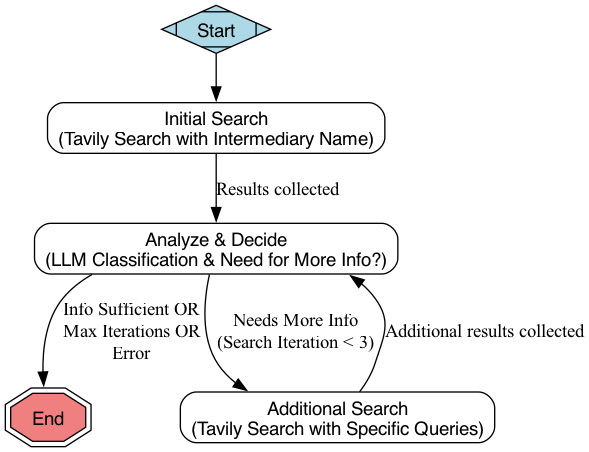
\includegraphics[width=0.8\textwidth]{agent_graph.png} 
    \caption{Agent Setup for Intermediary Classification}
    \label{fig:agent_loop_placeholder}
\end{figure}

In brief, the process involves an AI agent orchestrating online searches for each intermediary identified in the ICIJ data. It begins with generic searches, reads and interprets the initial results, and then formulates more specific search queries based on the information discovered or identified as lacking. This iterative process involves up to three search queries per intermediary, scouring the top 15 most relevant web results identified through query-result embedding similarity using the Tavily Search API (though the tool is relatively generic and it specifically is not very important). This effectively replaces the time-consuming need for manual searching of the intermediaries.

Based on the information gathered, the AI agent then classifies the intermediary according to the EU (2017) typology (Tax Expert, Legal Expert, Administrator, Investment Advisor), adding a few additional relevant fields (e.g., specific job title). Crucially, the agent also provides a confidence score for its classification judgment, allowing for filtering or weighting in subsequent analyses.

There are a few obvious limitations associated with this approach that warrant discussion:

Temporal Misalignment: A primary concern is that all online searches are conducted based on information available today, whereas the ICIJ data pertains to activities that may have occurred years or even decades prior. This introduces two potential issues:
    1.  The process might be biased towards identifying intermediaries who are still active or have a significant online presence currently.
    2.  It implicitly assumes that the role an intermediary plays today (as reflected online) is equivalent to the role they played at the time relevant to the ICIJ data.

Addressing the Limitations: While these issues are real, they are not prohibitive for their use in this thesis.
1. Regarding the first point (bias towards current intermediaries), this primarily impacts the coverage or statistical power of the classification – we may only be able to confidently classify a subset (e.g., 50\%) of all intermediaries. This is acceptable, provided the unclassifiable intermediaries are not systematically different in ways that correlate with the research questions. The issue becomes problematic only if there is a systematic bias in identifiability across types (e.g., if it is inherently much harder to find information online about legal experts compared to tax experts due to differing needs for discretion or public visibility).
2. Regarding the second point (role stability), the assumption that roles remain consistent is arguably less problematic. Given the highly specialized nature of functions like tax advisory, legal structuring, administration, and investment management within the offshore context, and the considerable barriers to entry (qualifications, reputation, networks) for each, frequent switching between these core roles by individuals or firms seems relatively unlikely.

In my view, it is the only pragmatically feasible method to do this given the constraints of this thesis.

(Note: LLMs have also been used to polish the text of this thesis.)

\chapter{Empirical Analysis}
\label{chap:empirical_analysis}

\section{Overview of the Dataset}
\label{subsec:overview_dataset}

This section provides an initial descriptive overview of the key structural characteristics that inform the subsequent, more focused and detailed analyses. 

\subsubsection{Concentration of Entities, Intermediaries, and Officers}

\label{subsubsec:concentration_elements}
A striking initial observation from the aggregated ICIJ dataset is the pronounced geographical concentration inherent in offshore financial activities, a characteristic that permeates all primary node types: entities, intermediaries, and officers.

While the dataset encompasses a vast network spanning over 200 countries and territories, these structures appear to be disproportionately concentrated within a relatively small cohort of key and recurring locations. Approximately 98.7\% of all entities within the dataset are legally registered in just 15 jurisdictions (see Figure \ref{fig:preliminary_geography_overview}, top-left panel). This aligns with the literature, such as Laffitte (2024), which suggests that Offshore Financial Centers (OFCs) often develop specialized expertise in particular 'legal technologies'-be it specific corporate vehicles like International Business Companies (IBCs), banking secrecy laws, or tax-exempt trusts. The British Virgin Islands, Panama, and the Bahamas, for instance, emerge as clear leaders in this regard, collectively accounting for a substantial majority of entity incorporations in the dataset.

This pattern of concentration, however, is not confined to the legal domiciliation of entities. It extends to the operational footprint of these entities and the intermediaries. As seen in the top-right panel, approximately 74\% of entities have their operational activities linked to the top 15 countries. These countries differ drastically, though, from the primary incorporation jurisdictions, featuring primarily the major financial centers such as Malta, Hong Kong, the United Kingdom, Switzerland, and Cyprus. This is to be expected as these same countries are highly linked to tax multinationals' tax avoidance. Malta and Hong Kong, for example, which rank first and second respectively for entity activity, also have exceptionally high ratios of corporate income tax revenues to national income, Malta being the highest, Hong Kong third (Saez and Zucman, 2019). 

The concentration extends to the intermediaries. The bottom-left panel of Figure \ref{fig:preliminary_geography_overview} shows that approximately 70.2\% of intermediaries are based in the top 15 countries. These include prominent financial centers like Hong Kong, the United Kingdom, Switzerland, the United States, and China. This resonates with the previously cited findings of Stausholm and Garcia-Bernardo (2024), who argue that the professional services underpinning the offshore world—legal, accounting, and financial advisory—tend to cluster in major global financial centers rather than exclusively in traditional tax havens. These hubs provide the necessary infrastructure, talent pool, and network access for intermediaries to orchestrate these structures.

Finally, the bottom-right panel indicates that around 61.5\% of officers are associated with the top 15 countries, with Hong Kong, China (excluding Hong Kong), the United Kingdom, Taiwan, and the United States being particularly prominent. As with intermediaries, this suggests that the individuals who hold positions of control or influence within these offshore entities are often based in the same major financial centers.

The varying degrees of concentration across these node types are also worth pointing out. The near-total concentration of entity incorporations (98.7\% in the top 15) contrasts with the more diffuse, yet still significant, concentration for active entities (74.0\%), intermediaries (70.2\%), and officers (61.5\%). This suggests that while the legal creation of offshore entities is highly centralized in a few specialized jurisdictions, the operational management, facilitation, and beneficial control of these entities are spread across a wider, though still limited, range of influential countries. This has both implications for what \textit{type} of chokepoints exist as well as to which \textit{extent}.

\begin{figure}[htbp]
    \centering
    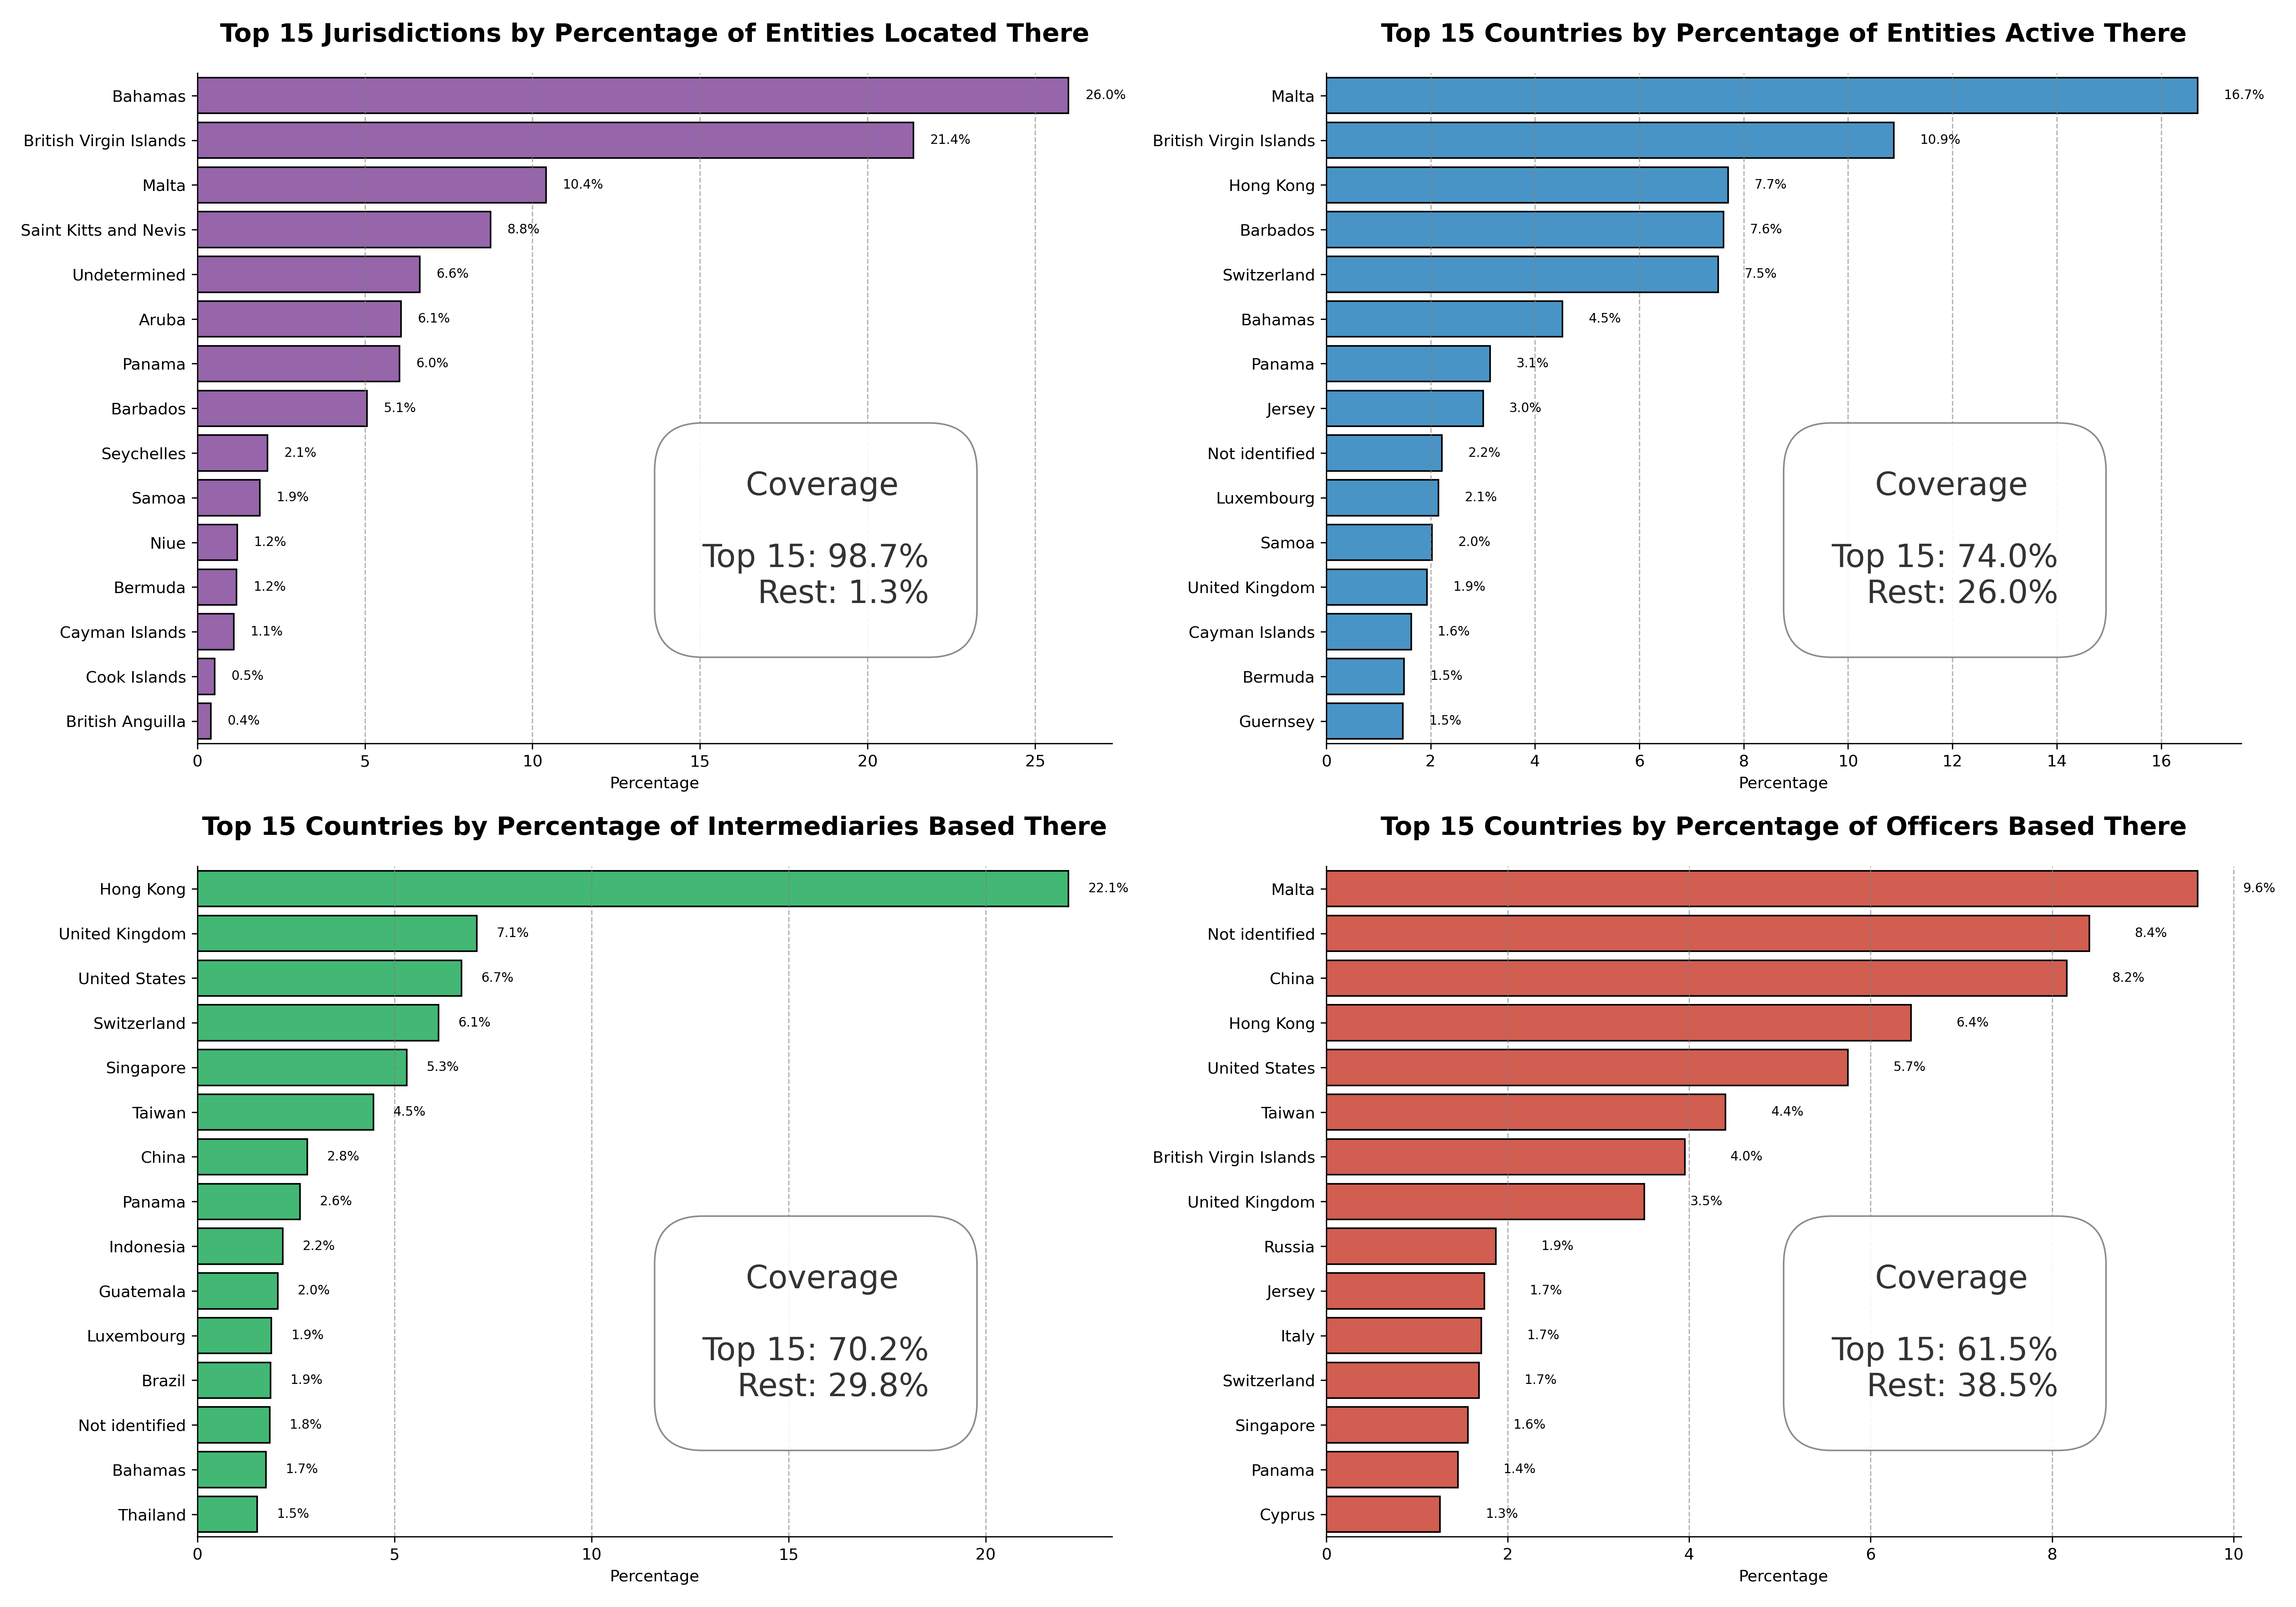
\includegraphics[width=0.9\textwidth]{images/Preliminary_Geography_Overview.png} 
    \caption{Geographical Concentration of Entities, Intermediaries, and Officers. Bar charts illustrate the percentage of total entities incorporated in the top 15 jurisdictions, entities with activity linked to the top 15 countries, intermediaries based in the top 15 countries, and officers associated with the top 15 countries.}
    \label{fig:preliminary_geography_overview}
\end{figure}

\section{Geographical Specialisation}
\label{sec:geographical_specialisation}

This section delves into the geographical patterns exhibited by intermediaries, focusing on the locations of the entities they service and the jurisdictions they select to incorporate in. We begin by examining specialization at the country level, analyzing how intermediaries based in specific nations in the aggregate, are concentrated in different and distinct countries. Subsequently, we shift to the individual intermediary level to investigate the concentration of their client networks and jurisdictional preferences.

\subsubsection{Intermediary Specialisation at the Country Level}
\label{subsubsec:intermediary_specialisation_country}

To understand how intermediaries based in specific countries orient their services, we examine two key dimensions: the geographical distribution of countries where the entities are primarily active, and the jurisdictions they predominantly use for incorporating these entities. Heatmaps are used to visually represent these patterns for intermediaries headquartered in the top 5 countries by intermediary count within the dataset: Hong Kong (HKG), Great Britain (GBR), the United States (USA), Switzerland (CHE) and Singapore (SGP). The rest of the top 15 (thus accounting for 70.2\% of all intermediaries as aforementioned) are left in the appendix, as well as Cyprus to illustrate the well-known Russia-Cyprus corridor, and how they manifest themselves in figures like these (e.g. Weinberg, 2023; Garcia-Bernado et al., 2017) 

Figures \ref{fig:geography_country_heatmaps_top5} display these heatmaps. Each panel within these figures corresponds to one of the top 5 intermediary home countries. The top bar in each panel illustrates the percentage distribution of client entities' countries of activity, while the bottom bar shows the percentage distribution of jurisdictions used for entity incorporation by intermediaries based in that home country. Darker shades indicate higher concentrations. Alongside each panel, normalized Shannon entropy values are provided for client country concentration ($H_c$) and incorporation jurisdiction concentration ($H_j$), where a value closer to 0 indicates higher concentration (less diversity) and a value closer to 1 indicates greater diversity.


\textbf{Figure \ref{fig:geography_country_heatmaps_top5} – Intermediaries in Top 1-5 Countries:}
This figure covers major global and regional financial centers.

\begin{itemize}
    \item \textbf{Hong Kong (HKG):} Intermediaries in Hong Kong predominantly serve entities active within Hong Kong itself (63\%), with a significant portion also linked to China (35\%). This strong domestic and near-regional focus ($H_c=0.23$) contrasts with their incorporation strategy. For incorporations, the British Virgin Islands (VGB) is overwhelmingly favored (78\%), followed by Samoa (WSM, 7\%) and the Cayman Islands (CYM, 6\%), resulting in a jurisdiction entropy ($H_j=0.33$) that, while still concentrated, indicates slightly more diversity than their client base. This pattern suggests HKG intermediaries leverage specific offshore jurisdictions like VGB for their largely local and Chinese clientele. In other words, a corroboration that Hong Kong intermediaries act as a gateway for Chinese to access offshore structuring, primarily through VGB (see, for example, Wei, 2024).

    \item \textbf{Great Britain (GBR):} UK-based intermediaries also show a strong domestic client focus (GBR, 73\%), with smaller but notable client links to Crown Dependencies like Jersey (JEY, 6\%) and the Isle of Man (IOM, not in top 5 shown but implied by "Other"). Their client country entropy ($H_c=0.37$) is relatively low. For incorporations, they too heavily rely on VGB (66\%), followed by Panama (PAN, 15\%) and the Bahamas (BHS, 13\%), yielding a jurisdiction entropy ($H_j=0.35$) similar to their client concentration. This suggests a model of serving primarily UK-based clients using a select few popular offshore jurisdictions.

    \item \textbf{United States (USA):} US-based intermediaries exhibit a very strong domestic client focus (USA, 71\%), with a low client country entropy ($H_c=0.24$). Their preferred incorporation jurisdictions are VGB (43\%), Panama (PAN, 19\%), and the Cook Islands (COK, 18\%), showing more jurisdictional diversity ($H_j=0.50$) than their client base. This indicates a strategy of serving predominantly American clients with a broader toolkit of offshore options.

    \item \textbf{Switzerland (CHE):} Swiss intermediaries show an exceptionally high concentration of domestic clients (CHE, 94\%), reflected in a very low $H_c=0.11$. This aligns with Switzerland's role as a wealth management hub primarily serving its own residents or those with assets managed through Swiss institutions. For incorporations, Panama (PAN, 50\%) and VGB (32\%) are dominant, leading to a moderate jurisdiction entropy ($H_j=0.45$).

    \item \textbf{Singapore (SGP):} Intermediaries in Singapore serve a mix of domestic (SGP, 47\%) and regional clients, particularly from Indonesia (IDN, not in top 5 shown but a known link). Their client country entropy ($H_c=0.32$) is moderate. Like Hong Kong, they overwhelmingly prefer VGB (84\%) for incorporations, resulting in a low jurisdiction entropy ($H_j=0.26$).
\end{itemize}

\begin{figure}[htbp]
    \centering
    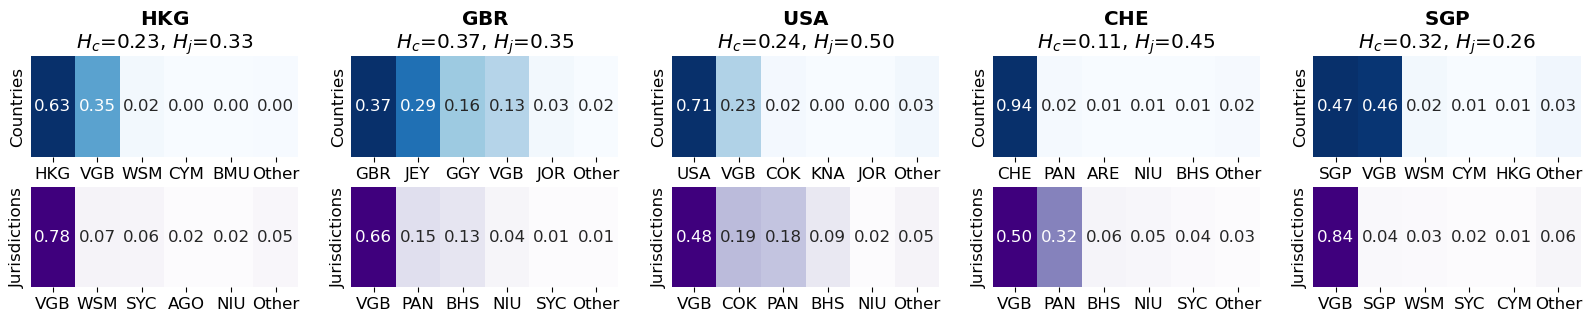
\includegraphics[width=0.9\textwidth]{images/Geography_Country_Heatmaps_Top5.png}
    \caption{Client and Incorporation Jurisdiction Heatmap for Intermediaries in Top 5 Countries (HKG, GBR, USA, CHE, SGP). Each panel shows the distribution of client entity countries (by activity, top bar) and incorporation jurisdictions (bottom bar) for intermediaries based in the specified country. $H_c$ denotes country entropy and $H_j$ denotes jurisdiction entropy for that group of intermediaries.}
    \label{fig:geography_country_heatmaps_top5}
\end{figure}

Across these five countries, a general trend emerges: intermediaries often have a geographically concentrated client base, frequently dominated by entities active in their own country of operation or in close regional proximity. However, their choice of incorporation jurisdictions tends to be more outwardly focused, though often dominated by a few key OFCs like the British Virgin Islands, Panama, and Seychelles. This suggests that while client acquisition may be localized or regionally focused, intermediaries draw from a global "market for tax havens" (Laffitte, 2024) to select specific "legal technologies" offered by these jurisdictions to meet diverse client structuring needs. Also notable to mention the generally lower entropy values for client countries compared to incorporation jurisdictions, indicating that intermediaries often operate within a narrower geographical scope for their clients than the range of jurisdictions they utilize for entity structuring. 

This observed difference in diversification is quantified by comparing the normalized entropy of jurisdictions used for incorporation ($H_j$) with the normalized entropy of client entity countries ($H_c$) at the aggregate level for intermediaries in all countries. Figure \ref{fig:geography_country_level_entropy_distribution} displays the distributions of these two entropy measures. The distribution of jurisdiction entropy (purple curve) is visibly to the right compared to the distribution of client country entropy (blue curve). A higher entropy value indicates greater diversification. Thus, intermediaries, when grouped by their country of operation, generally utilize a more diverse set of incorporation jurisdictions than the diversity observed in their clients' countries of activity. Given we are comparing two distributions, a two-sample Kolmogorov-Smirnov test confirms that these two distributions are statistically different (KS test: $p \approx 3 \times 10^{-7}$), providing robust evidence for this pattern. This confirms that while intermediaries' client acquisition strategies might be geographically focused, their operational toolkit for entity structuring draws upon a wider, more international palette of offshore jurisdictions.

\begin{figure}[htbp]
    \centering
    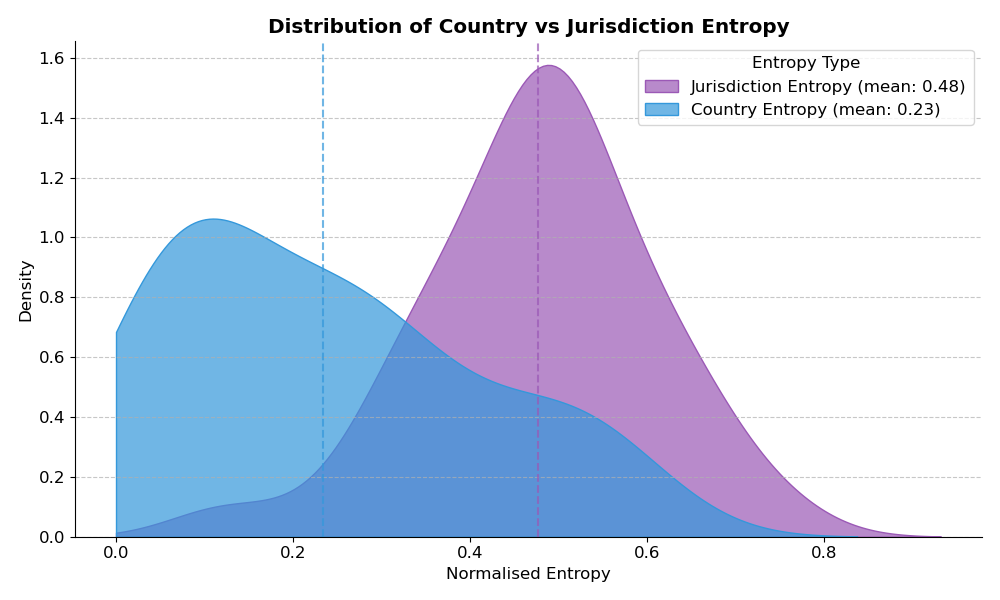
\includegraphics[width=0.8\textwidth]{images/Geography_Country_Level_Entropy_Distribution.png}
    \caption{Distribution of Normalized Entropy for Client Countries vs. Incorporation Jurisdictions, Aggregated at the Country Level of Intermediaries. The plot shows that intermediaries, when grouped by their country of operation, tend to use a more diverse set of incorporation jurisdictions ($H_j$, mean = 0.48) than the diversity observed in their clients' countries of activity ($H_c$, mean = 0.23). The dashed lines indicate the means of the distributions.}
    \label{fig:geography_country_level_entropy_distribution}
\end{figure}

\subsubsection{Intermediary Specialisation at the Individual Level}
\label{subsubsec:network_countries_served} 

While intermediaries aggregated at the country level exhibit distinct geographical specializations, particularly in their client bases, this section shifts focus to the individual intermediary level. We examine the concentration of countries linked to the entities an individual intermediary serves, and the range of jurisdictions they employ for incorporations.

Figure \ref{fig:geography_distribution_countries_by_intermediary} (left panel) presents the distribution of the number of distinct countries linked to the entities served by each intermediary. The distribution is heavily skewed to the right, with the vast majority of intermediaries (approximately 75\%) serving entities linked to only one country. More than 90\% of intermediaries serve entities linked to no more than two countries. This indicates that most individual intermediaries, regardless of their home country, focus their client acquisition efforts very narrowly, often within a single national context. The right panel of Figure \ref{fig:geography_distribution_countries_by_intermediary} plots the number of client countries against the log-degree of the intermediary (a proxy for the number of entities they serve). This scatter plot visually confirms a very low correlation: even intermediaries with a high degree (serving many entities) typically do not serve entities linked to a large number of different countries. This suggests that intermediaries tend to scale their operations by achieving deeper penetration within their existing client geographies rather than by expanding their client base across numerous new countries. This finding aligns with qualitative research suggesting that trust and local network knowledge are paramount in the client-intermediary relationship (Harrington, 2016), potentially favoring localized client acquisition.

\begin{figure}[htbp]
    \centering
    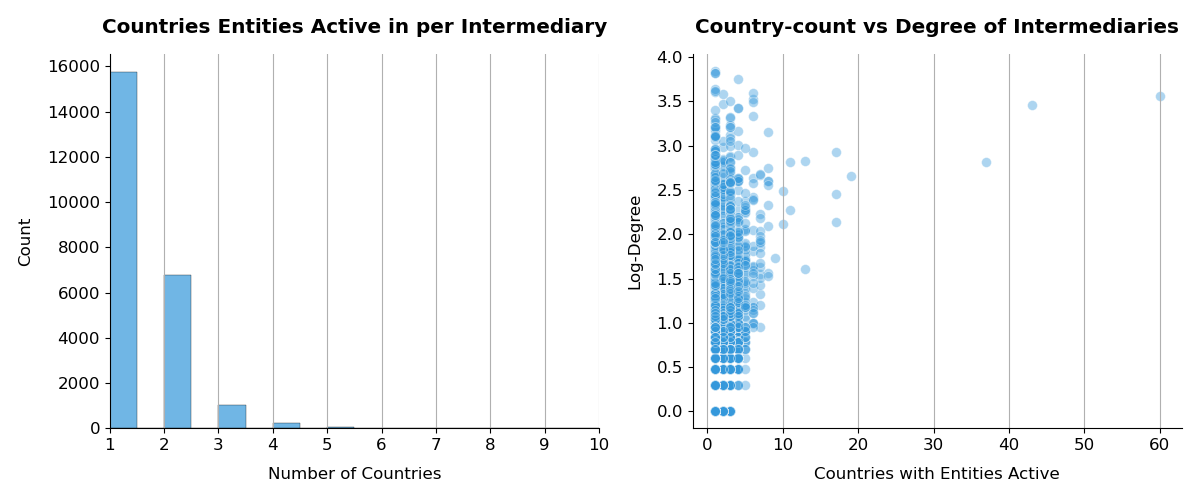
\includegraphics[width=0.9\textwidth]{images/Geography_Distribution_of_Countries_by_Intermediary.png} % Assuming this figure has two panels as described
    \caption{Left: Distribution of the Number of Countries Linked to Entities Served per Intermediary. Right: Scatter plot of Number of Countries vs. Log-Degree of Intermediary. The distribution is heavily skewed, with most intermediaries serving entities linked to only one or a few countries, even high-degree intermediaries.}
    \label{fig:geography_distribution_countries_by_intermediary}
\end{figure}

Turning to the jurisdictions used for incorporation, Figure \ref{fig:geography_distribution_jurisdictions_by_intermediary} (left panel) shows the distribution of the number of distinct jurisdictions each intermediary utilizes. Similar to the client country distribution, this is also heavily skewed, with most intermediaries (approximately 65\%) using only one jurisdiction for incorporating entities, and around 85\% using no more than two. This suggests that many intermediaries specialize in the "legal technologies" (Laffitte, 2024) of a very limited number of OFCs. However, comparing this to Figure \ref{fig:geography_distribution_countries_by_intermediary}, the skew appears slightly less extreme, hinting that some intermediaries might use a couple of jurisdictions even if their client base is from a single country. The right panel of Figure \ref{fig:geography_distribution_jurisdictions_by_intermediary} plots the number of jurisdictions used against the log-degree of the intermediary. While still showing considerable concentration, there is a discernible, albeit weak, positive trend: some intermediaries with very high degrees (top 1-5\%) do tend to utilize a broader portfolio of jurisdictions (e.g., 5 or more). This "tail" of highly connected intermediaries who also master a wider range of jurisdictional options may represent a distinct class of "super-enablers" within the offshore system, capable of offering more complex, multi-jurisdictional structuring (Christensen et al., 2022).

Overall, at the individual level, intermediaries exhibit strong specialization in their client-facing operations, primarily serving entities linked to one or two countries. While many also specialize in using only one or two incorporation jurisdictions, there is a tendency, particularly among larger intermediaries, to command a slightly broader repertoire of jurisdictional tools. This echoes the aggregate finding that the "palette" of incorporation jurisdictions is often wider than the geographical spread of clients, suggesting that even a geographically focused client base may have diverse structuring needs that intermediaries meet by drawing on different OFCs.

\begin{figure}[htbp]
    \centering
    \includegraphics[width=0.9\textwidth]{images/Geography_Distribution_of_Jurisdictions_by_Intermediary.png} % Assuming this figure has two panels
    \caption{Left: Distribution of the Number of Distinct Jurisdictions Used per Intermediary. Right: Scatter plot of Number of Jurisdictions vs. Log-Degree of Intermediary. Most intermediaries use only one or two jurisdictions for incorporation, but a tail of high-degree intermediaries uses a broader portfolio.}
    \label{fig:geography_distribution_jurisdictions_by_intermediary}
\end{figure}


\section{Functional Specialisation of Intermediaries}
\label{sec:functional_specialisation}

This section transitions from the geographical patterns of intermediary activity to the functional roles within the offshore financial ecosystem. The objective is to understand whether distinct operational characteristics align with established classifications of intermediary functions.  The analysis in this section primarily utilizes a classified random sample of intermediaries. 

\begin{figure}[htbp]
    \centering
    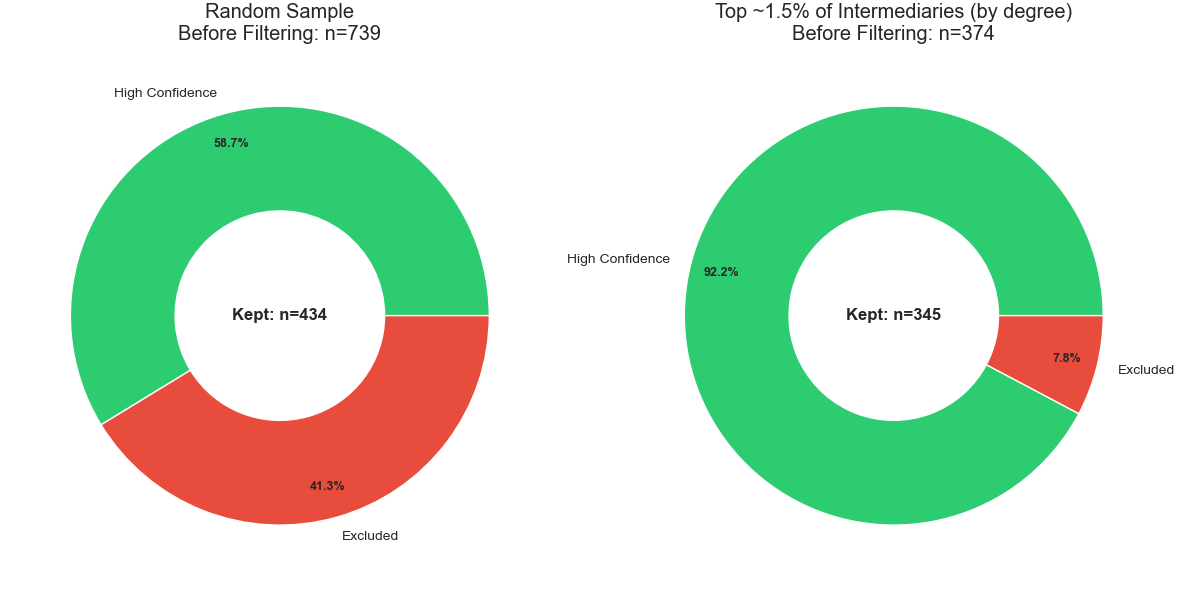
\includegraphics[width=0.6\textwidth]{Appendix_Filtering_of_Enrichment.png}
    \caption{Overview of the Iterative Filtering and Classification Process for the Random Sample of Intermediaries. This flowchart illustrates the steps taken to enrich and classify the random sample, from initial search to final classification, aiming for high-confidence functional type assignments (see Appendix \ref{sec:appendix_enrichment_filtering_details} for full details).}
    \label{fig:appendix_filtering_enrichment}
\end{figure}

\subsubsection{Different Levels of Connectivity: Personalised Advice vs. Aid in Incorporation}
\label{subsubsec:connectivity_functional}

A primary hypothesis in differentiating intermediary functions is that their scale of operation, proxied by their network degree (the number of distinct entities they are connected to), will vary systematically. Intermediaries providing bespoke, personalised advice-such as Tax Experts offering specialised tax planning or Investment Advisors structuring wealth management solutions-will likely serve a smaller number of clients. Conversely, intermediaries whose core function is the more standardized provision of entity incorporation and ongoing administration—such as Administrators and certain Legal Experts specialising in high-volume corporate services—are expected to exhibit higher degrees, indicative of a larger client load.

Figure \ref{fig:specialisation_cdf_degrees} presents the Cumulative Distribution Function (CDF) of degrees for each of the four intermediary classifications within our random sample, plotted on a log-scale - given the power-law distribution of degree earlier - to accommodate the wide range. The CDF indicates the proportion of intermediaries (y-axis) whose degree is less than or equal to a given value (x-axis). A curve shifted towards the top-left signifies generally lower degrees.

\begin{figure}[htbp]
    \centering
    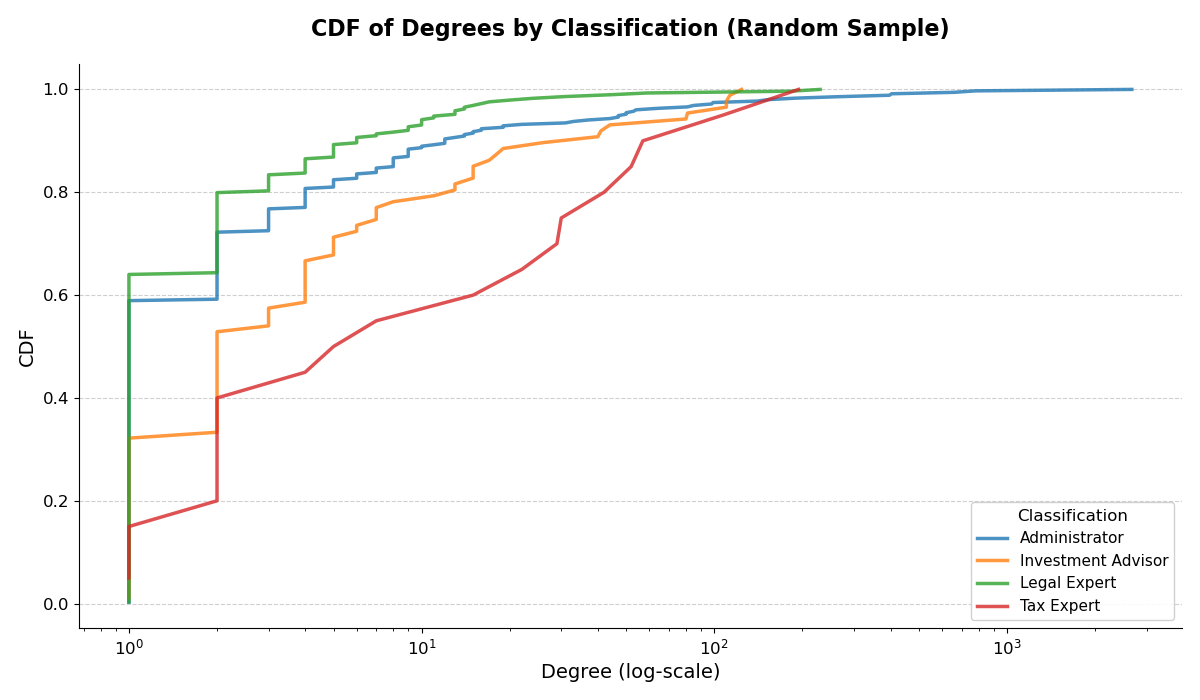
\includegraphics[width=0.8\textwidth]{Specialisation_CDF_of_Degrees_by_Classification_Random_Sample.png}
    \caption{Cumulative Distribution Function (CDF) of Degrees by Intermediary Classification (Random Sample). The x-axis (Degree) is on a log-scale. The plot shows distinct degree profiles, with Tax Experts and Investment Advisors generally having lower degrees (curves shifted top-left) than Administrators and Legal Experts (curves extending further right).}
    \label{fig:specialisation_cdf_degrees}
\end{figure}

The plot immediately suggests distinct degree profiles. The CDFs for Tax Experts (green line) and Investment Advisors (orange line) rise very steeply at the lower end of the degree spectrum, indicating that the vast majority of these intermediaries are connected to a relatively small number of entities (e.g., typically fewer than 10). Their curves plateau quickly, showing few instances of high-degree actors in these categories. In contrast, the CDFs for Administrators (blue line) and Legal Experts (red line) rise more gradually and extend further to the right, signifying a broader distribution of degrees, with a considerable proportion of these intermediaries connected to tens, hundreds, or even thousands of entities.

We are again dealing with comparing whether two distributions are significantly different, so we once again turn to the non-parametric two-sample KS test. However, two-sample test, so subsequent pairwise two-sample Kolmogorov-Smirnov (KS) tests were conducted, with a Bonferroni correction applied for multiple comparisons across the six unique pairs (corrected significance level $\alpha_c = 0.05/6 \approx 0.0083$).  

\begin{itemize}
    \item \textbf{Administrator vs. Investment Advisor:} A significant difference was found (KS = 0.267, $p_{corr} \approx 0.0024$), with Administrators exhibiting significantly higher degrees. This supports the hypothesis that administrative services are typically higher volume than bespoke investment advice.
    \item \textbf{Administrator vs. Legal Expert:} No significant difference was detected (KS = 0.077, $p_{corr} = 1.0000$). This suggests that, in terms of sheer connectivity, Administrators and Legal Experts in our sample operate at broadly similar scales, likely reflecting the involvement of many Legal Experts in high-volume incorporation and entity management tasks, similar to Administrators.
    \item \textbf{Administrator vs. Tax Expert:} A significant difference was observed (KS = 0.439, $p_{corr} \approx 0.0282$, although this p-value is above the strict Bonferroni threshold of 0.0083, it suggests a strong trend and is significant at a less stringent alpha). Administrators tend to have higher degrees than Tax Experts, consistent with tax advice being more specialised and lower volume.
    \item \textbf{Investment Advisor vs. Legal Expert:} A significant difference was found (KS = 0.318, $p_{corr} < 0.0001$), with Legal Experts having significantly higher degrees. This reinforces the distinction between high-volume legal/incorporation services and lower-volume investment advisory.
    \item \textbf{Investment Advisor vs. Tax Expert:} No significant difference was found (KS = 0.285, $p_{corr} = 1.0000$, original $p \approx 0.6899$). This lack of difference suggests that Investment Advisors and Tax Experts operate at comparable, generally lower scales of connectivity, consistent with their roles in providing personalised, in-depth advice rather than mass-produced services. This aligns with the idea that these professionals engage in more "strategic" action, tailoring solutions for individual clients (Christensen et al., 2022).
    \item \textbf{Legal Expert vs. Tax Expert:} A significant difference was detected (KS = 0.490, $p_{corr} \approx 0.0042$), with Legal Experts typically having higher degrees. This further distinguishes the often high-volume nature of legal services in this context from the more specialised, lower-volume nature of tax expertise.
\end{itemize}

These results broadly support the conceptual division: the "personalised advice" types (Tax Experts and Investment Advisors) tend to have lower degrees and do not significantly differ from each other in connectivity. The "aid in incorporation/management" types (Legal Experts and Administrators) tend to have higher degrees. Comparisons across these two broader functional groups generally reveal significant differences in their scale of operation. But we cannot distinguish between Legal Experts and Administrators in terms of degree, nor Tax Experts and Investment Advisors.

The importance of analysing a random sample, rather than focusing solely on the most connected intermediaries, is underscored by Figure \ref{fig:specialisation_classification_distribution}. This figure compares the distribution of intermediary classifications within our random sample (n=434 after filtering) against a sample composed of the top $\approx$1.5\% of intermediaries by degree (n=345 after filtering). The contrast is stark: the top-degree sample is overwhelmingly dominated by Administrators, who constitute 55.7\% of this group compared to 45.4\% in the random sample. Conversely, Legal Experts (22.6\% in top-degree vs. 29.0\% in random), Investment Advisors (19.1\% vs. 20.5\%), and particularly Tax Experts (a mere 2.6\% vs. 5.1\%) are notably underrepresented among the most connected players. This disparity highlights that an analysis focused only on "super-hub" intermediaries (Kejriwal \& Dang, 2020) would provide a limited and skewed perspective on the functional diversity within the offshore intermediary ecosystem, largely missing the contributions and characteristics of those providing more specialised, lower-volume advisory services. 

\begin{figure}[htbp]
    \centering
    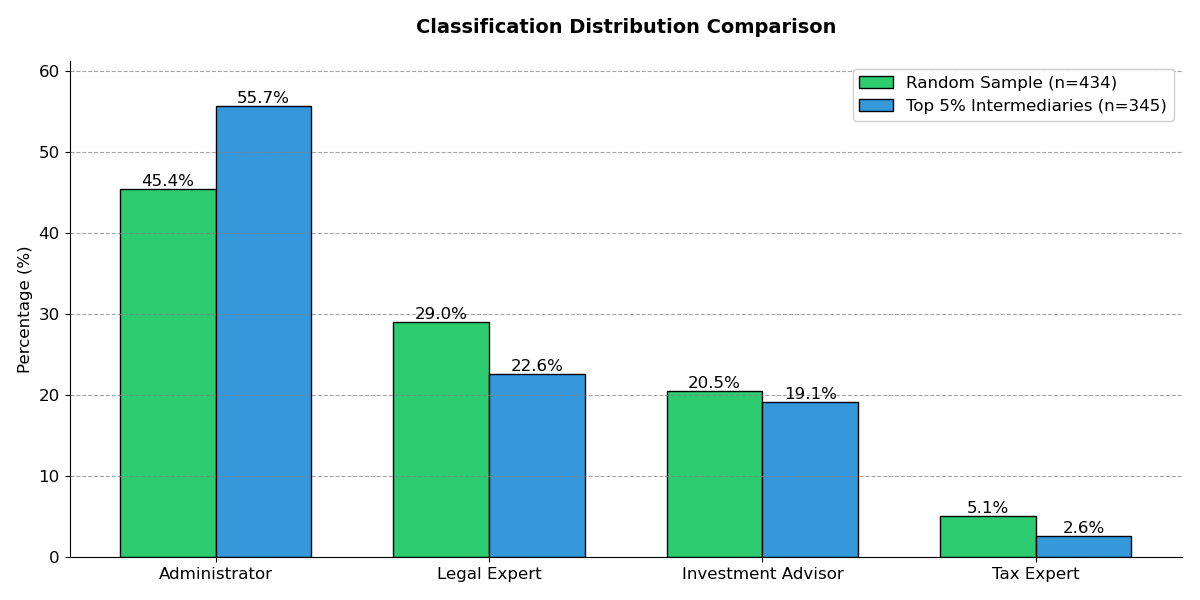
\includegraphics[width=0.8\textwidth]{Specialisation_Classification_Distribution_Comparison.png}
    \caption{Distribution of Intermediary Classifications: Random Sample vs. Top $\approx$1.5\% by Degree. The random sample (green bars, n=434) shows a more diverse mix of functional types compared to the top-degree sample (blue bars, n=345), which is heavily dominated by Administrators.}
    \label{fig:specialisation_classification_distribution}
\end{figure}

\subsubsection{Different Activities: Instruments and Service Offerings}
\label{subsubsec:activities_functional}

Beyond sheer connectivity, functional specialisation may also manifest in the nature and diversity of the activities intermediaries undertake. To explore this, we examine five key metrics for each intermediary classification within the random sample:
\begin{enumerate}
    \item \textbf{Jurisdiction Entropy ($H_j$)}: The diversity in the portfolio of jurisdictions where an intermediary incorporates entities. Higher entropy indicates the use of a wider range of jurisdictions.
    \item \textbf{Client Country Entropy ($H_c$)}: The diversity in the countries to which their clients' entities are linked (by activity). Higher entropy suggests a more geographically diverse client base.
    \item \textbf{Regime Entropy}: The diversity in the political regimes (e.g., democracy, autocracy, based on V-Dem data) of the countries where client entities are linked. Higher entropy implies engagement with clients from a broader spectrum of political systems.
    \item \textbf{Legal Technology Entropy}: The diversity in the types of "legal technologies" (as conceptualised by Laffitte, 2024, e.g., specific trust laws, corporate vehicles, secrecy provisions) prevalent in the jurisdictions they use for incorporation. Higher entropy suggests the intermediary leverages a wider array of legal tools available in the global "market for tax havens."
    \item \textbf{Bearer Instrument Usage}: A binary indicator (0 or 1) of whether the intermediary has serviced entities known to have used bearer instruments (e.g., bearer shares), which are high-anonymity tools often associated with obscuring beneficial ownership.
\end{enumerate}

Figure \ref{fig:specialisation_average_entropy_bearer} displays the average values of these metrics for each intermediary classification. Visually, Legal Experts and Administrators tend to show higher average values for most entropy measures, particularly Legal Technology Diversity and Jurisdiction Diversity, compared to Investment Advisors and Tax Experts. Bearer Share Usage appears relatively low across all types, with Tax Experts showing the highest average.

\begin{figure}[htbp]
    \centering
    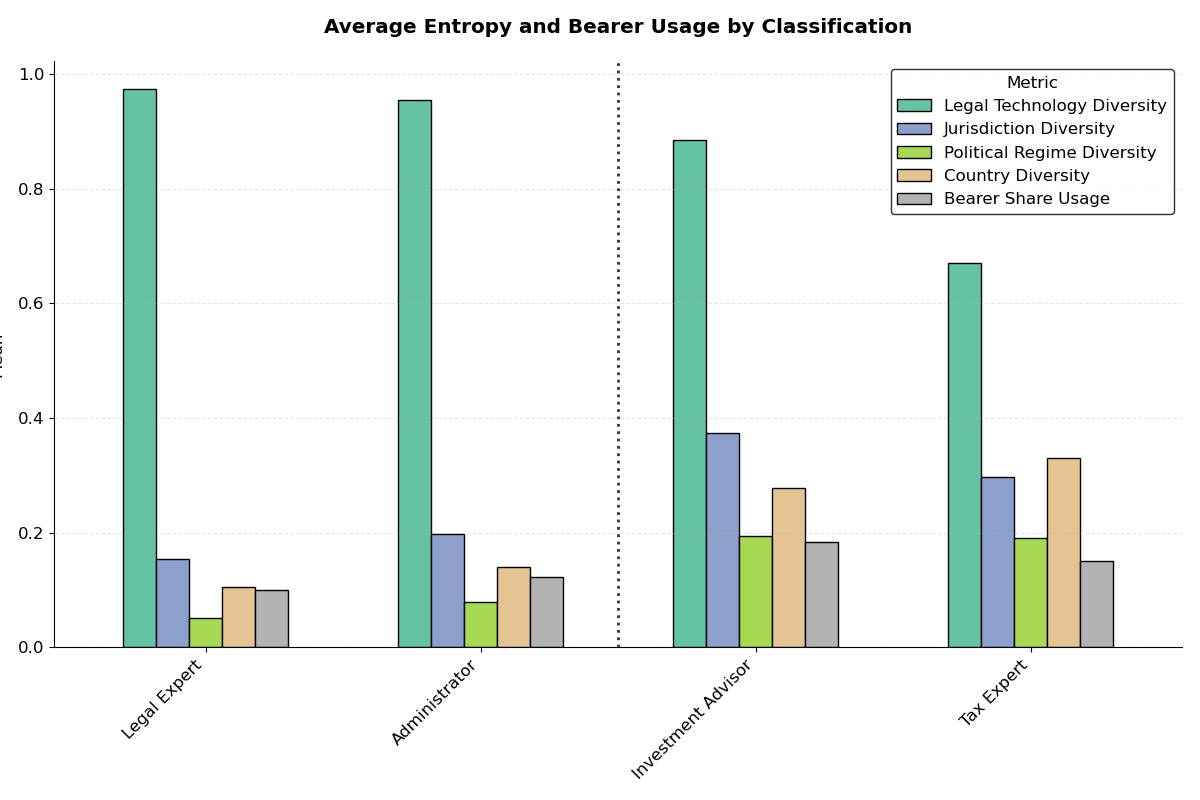
\includegraphics[width=0.9\textwidth]{Specialisation_Average_Entropy_and_Bearer_Usage_by_Classification.png}
    \caption{Average Entropy Measures and Bearer Instrument Usage by Intermediary Classification (Random Sample). Error bars represent standard errors of the mean. Higher entropy values indicate greater diversity. Bearer Share Usage is a proportion (0-1).}
    \label{fig:specialisation_average_entropy_bearer}
\end{figure}

To formally assess these differences, pairwise comparisons were conducted using Mann-Whitney U tests for the continuous entropy measures and Fisher's exact test for the binary bearer instrument usage. A Bonferroni correction was applied to account for the 30 comparisons (5 metrics $\times$ 6 unique pairs of classifications), setting the corrected significance threshold at $\alpha_c = 0.05/30 \approx 0.00167$. Key significant findings are summarized below, going measure by measure:

\textbf{Legal Technology Entropy:}
Legal Experts (mean $H_{LT} \approx 0.98$) and Administrators (mean $H_{LT} \approx 0.95$) exhibit significantly higher diversity in the legal technologies of the jurisdictions they utilize compared to Investment Advisors (mean $H_{LT} \approx 0.89$; $p_{corr} < 0.0001$ vs Legal Experts, $p_{corr} \approx 0.0047$ vs Administrators) and Tax Experts (mean $H_{LT} \approx 0.67$; $p_{corr} < 0.0001$ vs Legal Experts, $p_{corr} < 0.0001$ vs Administrators). This suggests that Legal Experts and Administrators, often involved in the mechanics of entity creation and management across various contexts, engage with a broader array of jurisdictional legal frameworks and offshore "products," as described by Laffitte (2024). No significant difference was found between Legal Experts and Administrators, nor between Investment Advisors and Tax Experts in this regard, reinforcing the two broad functional groupings proposed earlier.

\textbf{Jurisdiction Entropy:}
Legal Experts (mean $H_j \approx 0.15$) show significantly higher diversity in the jurisdictions they use for incorporation compared to Investment Advisors (mean $H_j \approx 0.04$; $p_{corr} < 0.0001$). Similarly, Administrators (mean $H_j \approx 0.20$) demonstrate greater jurisdiction diversity than Investment Advisors ($p_{corr} \approx 0.0012$). This indicates that Legal Experts and Administrators tend to draw from a wider palette of offshore jurisdictions when structuring entities for their clients, which aligns with their higher connectivity and broader operational scope. Other pairwise comparisons for jurisdiction entropy did not yield statistically significant differences after Bonferroni correction.

\textbf{Regime Entropy:}
Legal Experts (mean $H_{Regime} \approx 0.05$) exhibit significantly higher diversity in the political regimes of their client countries compared to Investment Advisors (mean $H_{Regime} \approx 0.02$; $p_{corr} < 0.0001$) and Tax Experts (mean $H_{Regime} \approx 0.02$; $p_{corr} \approx 0.0001$). Administrators (mean $H_{Regime} \approx 0.08$) also show significantly higher regime diversity than Investment Advisors ($p_{corr} \approx 0.0044$). This pattern suggests that Legal Experts and Administrators may cater to clienteles originating from, or structuring activities in, a more diverse set of political environments, potentially reflecting more internationalized operations.

\textbf{Client Country Entropy:}
Legal Experts (mean $H_c \approx 0.10$) demonstrate significantly higher diversity in their client countries compared to Investment Advisors (mean $H_c \approx 0.03$; $p_{corr} \approx 0.0001$) and Tax Experts (mean $H_c \approx 0.03$; $p_{corr} < 0.0001$). Administrators (mean $H_c \approx 0.14$) also have significantly more diverse client countries than Tax Experts ($p_{corr} \approx 0.0057$). This implies that Legal Experts, and to some extent Administrators, engage with clients whose activities span a broader range of countries, consistent with their roles in facilitating complex, multi-jurisdictional structures for a larger number of entities.

\textbf{Bearer Instrument Usage:}
After Bonferroni correction, \textbf{no statistically significant differences} were found in the propensity to use bearer instruments among any of the intermediary classifications (e.g., Administrator vs. Tax Expert, Fisher's exact $p_{corr} \approx 0.13$). While Tax Experts show a slightly higher raw average usage in Figure \ref{fig:specialisation_average_entropy_bearer}, this difference is not statistically significant. This suggests that, within this classified random sample, the use of these high-anonymity instruments is not strongly associated with a particular functional type of intermediary. Their seemingly non-specialised use might imply either a more diffuse deployment across the offshore industry for specific client needs.

The activity metrics, therefore, largely reinforce the distinctions observed in connectivity. Legal Experts and Administrators, typically more connected, also tend to exhibit greater diversity across various geographical, political regime, and legal-technical dimensions of their service offerings. This is consistent with their roles in high-volume incorporation and management, potentially serving more international and varied clienteles or requiring a broader toolkit of jurisdictional solutions. The "personalised advice" groups (Tax Experts and Investment Advisors), with their lower connectivity, generally appear more focused in these activity respects. 


\chapter{Discussion}
\label{chap:discussion}

\section{Three Propositions}

Three core propositions developed

Not in themselves particularly novel - none of them come as a particular surprise - but viewed through a set of new empirical data.
\subsection{Proposition 1: Specialisation of Intermediaries}

Functional Specialisation: Even though there's bound to be measurement error with the approach taken here, yet still significance for at least two distinct sets of roles. Taking outset from the typology of De Groen (2017). 

First set of roles:
\begin{itemize}
  \item Administrators
  \item Legal Experts
\end{itemize}

Second set:
\begin{itemize}
  \item Tax Experts
  \item Investment Advisors
\end{itemize}

\begin{itemize}
\item Both the significance of the degree distribution only between those two sets,
\item likewise entropy measures and bearer instrument share clearly visually distinct and significant across those two groups, but not very much within
\end{itemize}

Correlate with operational scale (degree of connectivity) and the diversity of their service portfolios (jurisdictional and legal-tech entropy). Personalised wealth management versus the mass provision of legal services.

Geographical Specialisation: Distinct development of preferential client corridors linking specific client origination countries to favored offshore jurisdictions, sometimes driven by historical ties, linguistic affinity, or specialized demand. As we'll see in proposition 3, still universal hubs that connect all these corridors.

\begin{itemize}
\item Country heatmaps,
\item Distribution of degree and country connections
\end{itemize}

\subsection{Proposition 2: Duality of Intermediary Focus - Local Anchors, Global Reach}

        Intermediaries often exhibit a primary client concentration within their own operational countries, likely leveraging local networks and trust (Granovetter, 1973; Stausholm, 2024; Harrington, 2016; Hoang, 2022). However, their core value proposition and a key driver of their specialization lies in their capacity to connect these local clients to a diversified global offshore architecture.
\begin{itemize}
\item Heatmaps showing intermediaries in HKG, GBR, USA etc., serving a notable portion of clients from their home country.
\item Lower client country entropy compared to jurisdiction entropy, suggesting more concentration in client origin.
\end{itemize}

\subsection{Proposition 3: Structural Centrality of Microstates in Intermediation Network}
A core set of Offshore Financial Centers (OFCs), that in heavy part are those infamous microstates. Highly central in it.

        Interesting to note, that this may also be due to their offering of versatile ``legal technologies'' like ``Dual-Purpose'' vehicles as for example is proposed in Laffitte (2024). Empirical confirmation that they form the structural backbone of the global offshore network, and are countries that intermediaries from all countries whose residents they do business and jurisdiction they incorporate. Critical hubs and bridges in chains of intermediation, facilitating complex offshore strategies regardless of client or intermediary home country.
\begin{itemize}
\item High centrality (betweenness, eigenvector) of jurisdictions like VGB, BHS, PAN, CYM, HKG in your co-service and co-usage networks.
\item Dominance of ``Dual-Purpose'' legal technologies in the central core of the jurisdiction co-usage network.
\item High lift values between key OFCs in association analysis.
\end{itemize}

\section{Implications for Regulation}

The potential to escape the multi-level games; most intermediaries serving officers in their own countries. Reclaiming lost tax revenue, can be done by targeting local citizens (though still the problem of changing citizenship).

Functional specialisation very much seeming to correlate with the degree: Layered due diligence or liability regimes could be interesting.

Affirming the centrality of microstates in the offshore network, and the potential for targeted regulation. Switzerland and Luxembourg as less active tax havens as case study.

And not least, affirming the importance of intermediaries.

\section{Limitations}

Where to begin. PLACEHOLDER

\section{Future Research}

\begin{itemize}
\item A lot within the current dataset that could be done - like extending a lot of the analyses. More importantly, the whole temporal dimension is currently left out; are the patterns persistent? As seen, network here has entities over a very large time frame, countless of them that are not active anymore.
\end{itemize}




\chapter{Conclusion}
\label{chap:conclusion}

This thesis covered an exploration of the often-shadowy world of offshore finance, not by chasing the beneficiaries, but by focusing on its architects: the intermediaries. We sought to understand how these crucial enablers specialize, asking \textit{how} they carve out their niches in a system that thrives on complexity and opacity. 

The core contention – that intermediaries exhibit significant geographical and functional specialization – finds robust support in the analysis. Geographically, many intermediaries are "local anchors with a global reach," deeply embedded in specific national or regional client markets, yet adept at navigating the global "supermarket" of offshore jurisdictions and their varied "legal technologies." This duality is key to their value proposition. Functionally, the data sketches distinct profiles: the high-volume "commoditizers" like many Administrators and Legal Experts, building broad infrastructures of entities, stand in contrast to the more bespoke "customizers" like Tax Experts and Investment Advisors, who offer tailored, often lower-volume, strategic counsel. These are not merely descriptive categories; they point to different operational logics, different scales of connectivity, and potentially different vulnerabilities.

The implications for those engaged in the "race" against tax avoidance are considerable. If intermediaries are indeed locally anchored, national regulators may possess more direct leverage than often perceived, offering a route to bypass the multi-level game of international tax governance. Furthermore, recognizing functional differentiation allows for more nuanced regulatory strategies - perhaps layered liability or tailored due diligence - rather than a one-size-fits-all approach.



%TC:ignore
% --- Appendix ---
\appendix
\chapter{Appendix}
\label{chap:appendix}

The hardest part - which I speak confidently on with my 21 years of experience on this earth - is always leaving material on the cutting-floor. I've, however, not had the willpower to completely relinquish this section of my thesis, and so with the brazen immaturity of a Bachelor's student, I've put it here, in vain hope that efforts won't feel wasted. 

The appendix is structured as follows. First, detailing a third proposition on the centrality of Microstates in Co-service networks of intermediaries in both countries and jurisidictions. Secondly, the empirical analysis behind it, in which, I will briefly discuss methods, then followed by the results of looking at these "co-service networks" of intermediaries across countries. Thirdly, I'll go a bit deeper on the method by which I've classified intermediaries using a novel agentic method.

\section{Proposition 3: Structural Centrality of Microstates in Intermediation Network}
A core set of Offshore Financial Centers (OFCs), that in heavy part are those infamous microstates. Highly central in it.

Interesting to note, that this may also be due to their offering of versatile ``legal technologies'' like ``Dual-Purpose'' vehicles as for example is proposed in Laffitte (2024). Empirical confirmation that they form the structural backbone of the global offshore network, and are countries that intermediaries from all countries whose residents they do business and jurisdiction they incorporate. Critical hubs and bridges in chains of intermediation, facilitating complex offshore strategies regardless of client or intermediary home country.

Looking at the central actors in these networks of countries that intermediaries make use of. This is where network analysis shines, with its cohsive langauge of ``centrality'' and ``community detection''.

\begin{itemize}
\item High centrality (betweenness, eigenvector) of jurisdictions like VGB, BHS, PAN, CYM, HKG in your co-service and co-usage networks.
\item Dominance of ``Dual-Purpose'' legal technologies in the central core of the jurisdiction co-usage network.
\item High lift values between key OFCs in association analysis.
\end{itemize}

\section{Concepts from Network Analysis}
\label{subsec:network_theory_concepts}

Specifically, network analysis is employed here to uncover the roles intermediaries play based on their positions within the interconnected offshore financial system revealed by the ICIJ data. As described in Section \ref{sec:3_1}, the ICIJ data forms a multi-modal graph (comprising entities, officers, intermediaries, etc.). Directly applying many standard network analysis concepts to such a multipartite graph can be challenging. Therefore, our approach often involves analyzing specific projections or subsets of the global graph to make the analytical tools from network theory applicable. The foundational textbook by Newman (2010) serves as the primary reference for this section.

\begin{itemize}
    \item \textbf{Centrality Scores}: To identify nodes of critical importance within specific network representations, we utilize two fundamental centrality measures. In the context of understanding the key countries for intermediary activity, these measures are applied to a network derived from intermediary incorporation patterns.
    \begin{itemize}
        \item \textbf{Eigenvector Centrality}: This measure assigns scores to nodes based on the principle that connections to high-scoring nodes contribute more to the score of the node in question than equal connections to low-scoring nodes. It is calculated as the principal eigenvector of the adjacency matrix $\mathbf{A}$ of the network, satisfying $x_i = \frac{1}{\lambda} \sum_{j} A_{ij} x_j$, where $x_i$ is the centrality score of node $i$, $A_{ij}$ is 1 if node $i$ is connected to node $j$ and 0 otherwise (or the weight of the edge), and $\lambda$ is the largest eigenvalue of $\mathbf{A}$ (cf. Perron-Frobenius theorem). Eigenvector centrality is chosen for its ability to identify nodes that are influential not just by having many connections, but by being connected to other influential nodes, providing a robust reading of which countries are most central in the network of intermediary incorporations.
        \item \textbf{Betweenness Centrality}: This metric quantifies the extent to which a node lies on shortest paths between other pairs of nodes. For a node $v$, it is defined as $C_B(v) = \sum_{s \neq v \neq t} \frac{\sigma_{st}(v)}{\sigma_{st}}$, where $\sigma_{st}$ is the total number of shortest paths between nodes $s$ and $t$, and $\sigma_{st}(v)$ is the number of those paths that pass through $v$. Betweenness centrality is used here to gauge which countries act as crucial "bridges" or conduits within the network, potentially connecting otherwise disparate segments, a role distinct from simply being a high-degree hub.
    \end{itemize}

    \item \textbf{Community Detection: Modularity Maximization}: To uncover clusters or communities of closely related nodes within the country network, we employ modularity maximization. This approach provides an atheoretical method for identifying densely connected groups of countries, which may reflect underlying similarities in how intermediaries utilize them. Such clustering could be influenced by factors like shared regime types (Chang et al., 2023c) or the trust dynamics inherent in relational capitalism. While traditional clustering algorithms could be applied, defining a meaningful distance or dissimilarity metric for nodes in these networks is non-trivial. Modularity maximization, conversely, assesses the quality of a partition by comparing the number of intra-community edges to what would be expected in a random network with similar properties (a null model). The quality of a partition $C$ is measured by the modularity $Q$:
    \begin{equation}
        Q = \frac{1}{2m} \sum_{i,j} \left[ A_{ij} - P_{ij} \right] \delta(c_i, c_j)
    \end{equation}
    where $m$ is the total number of edges, $A_{ij}$ is the actual weight of the edge between nodes $i$ and $j$, $P_{ij}$ is the expected weight of an edge between $i$ and $j$ under the Newman-Girvan null model (a configuration model preserving the degree sequence, where $P_{ij} = \frac{k_i k_j}{2m}$ for unweighted graphs, $k_i$ being the degree of node $i$), and $\delta(c_i, c_j)$ is 1 if nodes $i$ and $j$ are in the same community ($c_i=c_j$) and 0 otherwise. Since finding the optimal partition is an NP-hard (although, to be honest, at the size we reduce our graph sizes, search space isn't an issue...) problem, we utilize the Louvain method (Blondel et al., 2008), an efficient and widely adopted greedy algorithm, as implemented in the \texttt{networkx} library.

    \item \textbf{Power-law Distribution}: The distribution of node degrees (number of connections) and other network properties are examined for characteristics of power-law distributions. A power law, $P(k) \sim k^{-\alpha}$, describes a "fat-tailed" distribution where a few nodes (hubs) have a disproportionately high number of connections, while most nodes have few. Such distributions are frequently observed in real-world networks (Clauset et al., 2009; Kejriwal \& Dang, 2020) and their presence can indicate significant heterogeneity in node importance.

    \item \textbf{Density of a Graph}: Network density, the ratio of actual edges to the total number of possible edges in the network ($D = \frac{L}{N(N-1)/2}$ for an undirected graph with $L$ edges and $N$ nodes), is used to measure the general level of connectedness. Low density is typical for large, sparse networks and indicates that connections are selective rather than ubiquitous.
\end{itemize}

\section{Association Analysis}
\label{subsec:unsupervised_learning}
In line with the highly exploratory nature of this thesis, unsupervised learning techniques are employed to discover notable patterns within the data. Association analysis (Hastie et al., 2009) is particularly opportune for identifying non-obvious relationships or co-occurrences in large datasets, such as the ICIJ networks. For example, it can help determine which connections (e.g., between a type of intermediary and the use of a specific jurisdiction or legal technology) are particularly remarkable. This approach relies on a \textbf{non-parametric notion} of pattern discovery, aiming to \textbf{discover patterns of high density} or co-occurrence.

Two main tools from association analysis, based on simple set-theoretical notions, are used:
\begin{itemize}
    \item \textbf{Support}: This measures the overall frequency of an itemset (e.g., a specific attribute or combination of attributes) in the dataset. For an itemset $X$, $Support(X) = P(X) = \frac{\text{count}(X)}{N}$, where $N$ is the total number of transactions (e.g., intermediaries). For an association rule $A \rightarrow B$, $Support(A \rightarrow B) = P(A \cup B)$.
    \item \textbf{Lift}: This measures how much more likely item $B$ is to be present when item $A$ is present, compared to the baseline probability of $B$. It indicates the strength of an association beyond what would be expected by chance.
    \begin{equation}
        Lift(A \rightarrow B) = \frac{P(B|A)}{P(B)} = \frac{Support(A \cup B)}{Support(A) \times Support(B)}
    \end{equation}
    A lift value greater than 1 suggests a positive association, a value less than 1 suggests a negative association, and a value of 1 suggests independence. \textbf{Lift scores} will be used to quantify the strength of associations found, indicating, for example, how much more likely an intermediary of a certain type is to use a specific jurisdiction compared to the overall likelihood.
\end{itemize}




\section{Patterns of Co-Specialisation}
To explore these co-service relationships further, a network of countries was constructed. In this network, countries are nodes, and an edge exists between two countries if at least one intermediary serves clients (entities) linked to both. The weight of the edge reflects the number of distinct intermediaries serving clients in both countries. The resulting full country network consists of 121 nodes (countries) and 2,716 edges. Key summary statistics for this network are presented in Table \ref{tab:country_network_summary}. 

\begin{table}[htbp]
\centering
\caption{Summary Statistics for the Full Country Co-Service Network}
\label{tab:country_network_summary}
\begin{tabular}{lc}
\toprule
\textbf{Metric}                        & \textbf{Value}    \\
\midrule
Number of Nodes               & 121      \\
Number of Edges               & 2716     \\
Network Density               & 0.3741   \\
Average Degree                & 44.89    \\
Average Clustering Coefficient & 0.7728   \\
\bottomrule
\end{tabular}
\end{table}

Visualising such dense graphs is incredibly challenging - and to be entirely honest, the rest of the thesis could be filled with differently filtered versions of this graph, illuminating some other aspect of it. Therefore, to identify the most important connections, the network was filtered using principles from association analysis. Edges are displayed only if they 1) meet a minimum support threshold (representing at least 0.008 of all intermediaries' country-pair connections, meaning the pair is co-serviced by at least that fraction of intermediaries who service multiple countries) and 2) a lift score of 1.5 or higher. Lift measures how much more frequently two countries are co-serviced than would be expected if their servicing by intermediaries were independent. This filtering ensures that the visualized connections are not only reasonably frequent but also represent associations significantly stronger than chance, that they are both common links as well as carrying statistical signal. The resulting filtered network, or "backbone," thus highlights the most robust and significant co-service relationships. While the exact number of nodes included is sensitive to the choice of the lift and support thresholds here, this "backbone" as I term it, is relatively stable across a range of thresholds.

The nodes in the network visualization (Figure \ref{fig:geography_cross_country_network}) are coloured in two ways: first, by communities identified using the Louvain modularity maximization algorithm (Blondel et al., 2008), which groups densely interconnected countries; and second, by regime type using VDem data, as described in Section \ref{sec:3_2}. This dual coloring was intended to explore whether regime type influences intermediary operations and co-service patterns, a factor suggested by literature on offshore secrecy strategies (e.g. Chang et al., 2023b).

\begin{figure}[htbp]
    \centering
    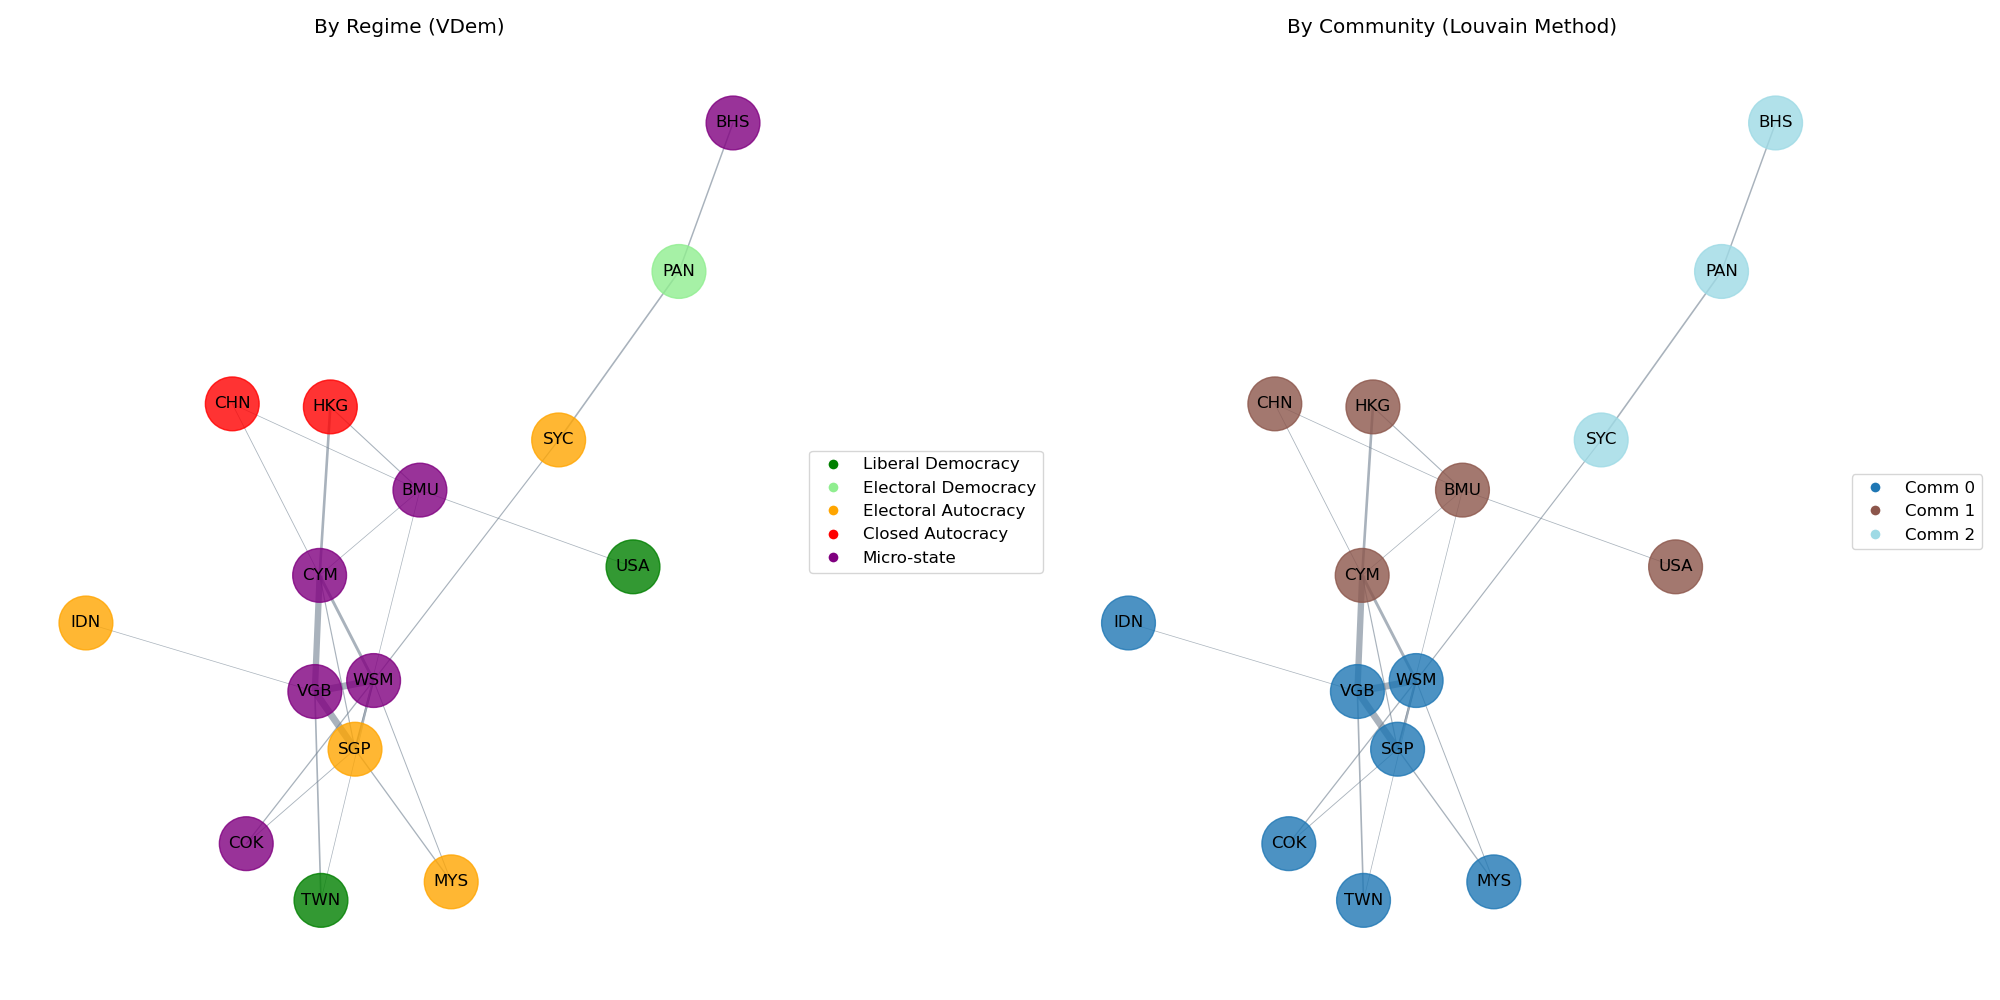
\includegraphics[width=0.9\textwidth]{Geography_Cross_Country_Network.png}
    \caption{Filtered Network of Co-Served Countries, Coloured by Louvain Community (left legend) and Regime Type (right legend). Edges shown have support $\ge 0.008$ and lift $\ge 1.5$. Node size can be proportional to degree or another centrality measure.}
    \label{fig:geography_cross_country_network}
\end{figure}

\paragraph{Interpretation of the Filtered Country Network Structure}
The filtered network (Figure \ref{fig:geography_cross_country_network}) reveals a sparse yet highly structured set of relationships, forming a distinct core-periphery structure. A central core of interconnected nodes is evident, particularly involving VGB (British Virgin Islands), CYM (Cayman Islands), and SGP (Singapore), along with their strong links to HKG (Hong Kong) and BMU (Bermuda).

When coloured by regime type, no clear large-scale clustering emerges that aligns strictly with political systems. The central cluster itself is diverse, including Micro-states (VGB, CYM, BMU), jurisdictions classified as Closed Autocracies (HKG, reflecting its unique status), and Electoral Autocracies (SGP). Liberal Democracies such as the USA and TWN (Taiwan) are present but connect to nodes of various different regime types. This visual evidence supports the notion that regime type, while potentially a factor in individual elite choices (Chang et al., 2023c), is not a primary driver of these strong, systemic co-service relationships at the country-network level. Economic roles, historical ties, and financial infrastructure likely play more dominant roles in shaping this backbone.

The Louvain community detection method, which is data-driven, reveals distinct groupings based on the density of co-service links:
\begin{itemize}
    \item \textbf{Community 0 (Dark Blue):} This is the largest community, featuring prominent offshore centers like VGB and CYM, major Asian economies/financial hubs like SGP, TWN (Taiwan), MYS (Malaysia), IDN (Indonesia), and Pacific jurisdictions like COK (Cook Islands) and likely WSM (Samoa, if present in the filtered graph). This highlights strong ties between several offshore financial centers and key Asian economies.
    \item \textbf{Community 1 (Brown):} This community comprises major economies like the USA and CHN (China), alongside HKG (Hong Kong) and the offshore jurisdiction BMU (Bermuda), indicating a distinct Atlantic-Pacific nexus involving Bermuda.
    \item \textbf{Community 2 (Light Blue):} A smaller, distinct community consisting of PAN (Panama), SYC (Seychelles), and BHS (Bahamas), all of which are significant offshore jurisdictions.
\end{itemize}
Most nodes in this backbone network are connected within two to three steps, indicating a relatively compact structure despite the filtering.

Centrality metrics calculated on the full 121-node co-service network (detailed in Appendix Tables \ref{tab:appendix_country_betweenness_app} and \ref{tab:appendix_country_eigenvector_app}) identify key players.
\textbf{VGB (British Virgin Islands)} is dominant, exhibiting the highest betweenness and eigenvector centrality, underscoring its pivotal role in connecting diverse client countries through shared intermediaries. The \textbf{USA} ranks second in both measures, reflecting its economic importance and the global reach of its client base serviced by international intermediaries. The USA is linked to BMU (Bermuda) in the filtered graph's Community 1. \textbf{HKG (Hong Kong) \& CHN (China)} also feature prominently in centrality scores and are central to Community 1. Numerous \textbf{Micro-states} (BMU, BHS, CYM) show high centrality, consistent with their specialized roles in offshore finance. \textbf{SGP (Singapore)} is another key, highly central node, bridging various parts of the network. In general, high centrality in the full network translates to a significant structural role in this filtered backbone, indicating that the most connected countries in the overall system also form the core of the strongest co-service relationships.

\paragraph{Significant Country Associations}
Lift scores from the association analysis (top associations detailed in Appendix Table \ref{tab:appendix_significant_country_associations_app}, filtered for co-occurrences $\ge 20$) reveal particularly strong and statistically significant pairings, many of which are visualized in Figure \ref{fig:geography_cross_country_network} (those with lift $\ge 1.5$).
Key findings include:
\begin{itemize}
    \item Strong \textbf{Micro-state synergies} are evident. For instance, the WSM-CYM (Samoa-Cayman Islands) pairing shows a high lift of 6.78, and VGB-CYM (British Virgin Islands-Cayman Islands) has a lift of 1.91. These indicate that intermediaries servicing clients in one of these micro-states are substantially more likely to also service clients in the other, suggesting complementary service offerings or established pathways for specific client types. The CYM-BMU (Cayman Islands-Bermuda) link is exceptionally strong with a lift of 13.5.
    \item A critical \textbf{China-Bermuda nexus} emerges with CHN-BMU showing a very high lift of 15.3. This suggests Bermuda acts as a particularly favored intermediary hub for clients linked to China. This is complemented by the USA-BMU link (lift 4.92), highlighting Bermuda's role in Community 1 of the filtered network, connecting major economic powers.
    \item Robust \textbf{Asian connections} are underscored by pairs like SGP-MYS (Singapore-Malaysia, lift 5.27). Singapore (SGP) also shows strong co-service patterns with various Micro-states such as WSM (Samoa, lift 3.04) and CYM (Cayman Islands, lift 3.89), reinforcing its role as a key hub in Community 0.
    \item A distinct \textbf{PAN-SYC-BHS nexus} (Community 2) is confirmed with pairings like PAN-SYC (Panama-Seychelles) having a lift of 3.89.
    \item Crucially, high lift values are common \textbf{across different regime types}. For example, China (Closed Autocracy) has a very high lift with Bermuda (Micro-state), and the USA (Liberal Democracy) also has a significant lift with Bermuda. This reinforces the earlier observation that factors beyond regime similarity, such as specialized financial services, established legal and commercial pathways, or historical ties, are potent drivers of these strong co-service relationships.
\end{itemize}

\subsubsection{Network of Jurisdictions Used by Intermediaries}
\label{subsubsec:network_jurisdictions_used}

Shifting focus from client locations to incorporation locations, this section analyzes the network of jurisdictions that intermediaries use in combination. The full jurisdiction co-usage network, where an edge exists if an intermediary incorporates entities in both jurisdictions (weighted by the number of such intermediaries), comprises 41 nodes and 347 edges. Summary statistics are provided in Table \ref{tab:jurisdiction_network_summary}. The distribution of the number of distinct jurisdictions used per intermediary is shown in Figure \ref{fig:geography_distribution_jurisdictions_by_intermediary}, indicating that most intermediaries utilize a small portfolio of jurisdictions, though some use many.

\begin{table}[htbp]
\centering
\caption{Summary Statistics for the Full Jurisdiction Co-Usage Network}
\label{tab:jurisdiction_network_summary}
\begin{tabular}{lc}
\toprule
\textbf{Metric}                        & \textbf{Value}    \\
\midrule
Number of Nodes               & 41       \\
Number of Edges               & 347      \\
Network Density               & 0.4232   \\
Average Degree                & 16.93    \\
Average Clustering Coefficient & 0.8155   \\
\bottomrule
\end{tabular}
\end{table}

\begin{figure}[htbp]
    \centering
    \includegraphics[width=0.8\textwidth]{Geography_Distribution_of_Jurisdictions_by_Intermediary.png}
    \caption{Distribution of the Number of Distinct Jurisdictions Used per Intermediary. Most intermediaries use only one or two jurisdictions for incorporation, but a tail of intermediaries uses a broader portfolio.}
    \label{fig:geography_distribution_jurisdictions_by_intermediary}
\end{figure}

Figure \ref{fig:geography_cross_jurisdiction_network} presents a filtered "backbone" of these co-usage patterns, applying the same support ($\ge 0.008$) and lift ($\ge 1.5$) thresholds as for the country co-service network. Nodes are coloured by their predominant legal technology profile (derived from Laffitte, 2024, as detailed in Section \ref{sec:3_2}) and by Louvain communities. The image displays the most prominent nodes in this filtered network, including CRI (Costa Rica), SGP (Singapore), CYP (Cyprus), GBR (Great Britain), BLZ (Belize), AGO (Angola), HKG (Hong Kong), CYM (Cayman Islands), COK (Cook Islands), MYS (Malaysia), BHS (Bahamas), SYC (Seychelles), PAN (Panama), NIU (Niue), WSM (Samoa), and USA.

\begin{figure}[htbp]
    \centering
    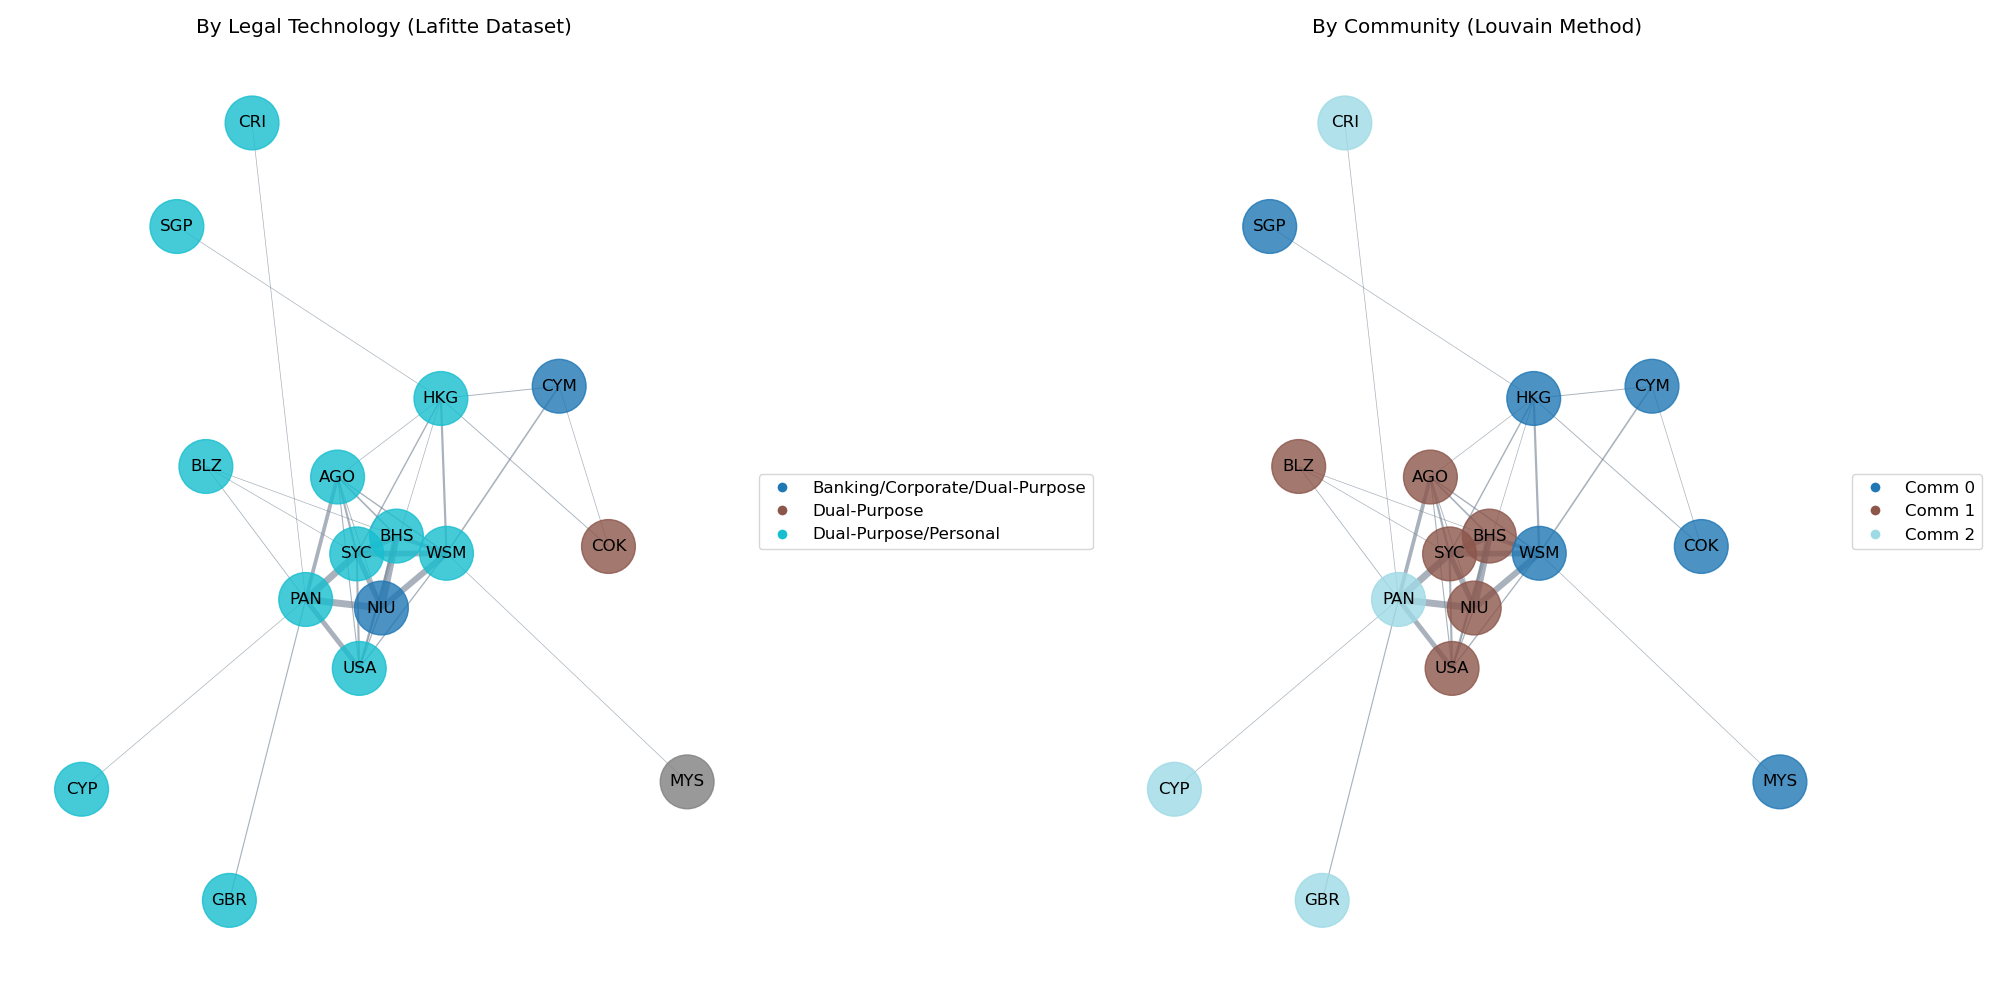
\includegraphics[width=0.9\textwidth]{Geography_Cross_Jurisdiction_Network.png}
    \caption{Filtered Network of Co-Used Jurisdictions, Coloured by Predominant Legal Technology (left legend) and Louvain Community (right legend). Edges shown have support $\ge 0.008$ and lift $\ge 1.5$.}
    \label{fig:geography_cross_jurisdiction_network}
\end{figure}

\paragraph{Interpretation of the Filtered Jurisdiction Network Structure}
The filtered jurisdiction network (Figure \ref{fig:geography_cross_jurisdiction_network}) reveals a central, densely connected core. Key jurisdictions in this core include BHS (Bahamas), SYC (Seychelles), AGO (Angola), WSM (Samoa), NIU (Niue), PAN (Panama), USA, and HKG (Hong Kong).

When coloured by their predominant legal technology profile (Laffitte, 2024), the central cluster is overwhelmingly dominated by jurisdictions offering \textbf{"Dual-Purpose"} legal technologies (e.g., International Business Companies - IBCs). This strongly supports the observation that central jurisdictions in this co-usage network are those providing flexible, widely applicable corporate vehicles suitable for both corporate and personal wealth structuring. 

Louvain community detection identifies the following groupings based on co-usage patterns:
\begin{itemize}
    \item \textbf{Community 1 (Brown):} This is the largest and most central community, encompassing jurisdictions like USA, PAN, NIU, BHS, SYC, AGO, and WSM. These are largely characterized by "Dual-Purpose" legal technologies.
    \item \textbf{Community 0 (Dark Blue):} This community includes HKG, CYM (Cayman Islands), and COK (Cook Islands), combining jurisdictions known for "Banking/Corporate/Dual-Purpose" (like HKG) with those strong in "Dual-Purpose/Personal" (like CYM, COK).
    \item \textbf{Community 2 (Light Blue):} This community is more peripheral in the filtered network and includes SGP (Singapore), CRI (Costa Rica), CYP (Cyprus), GBR (Great Britain), BLZ (Belize), and MYS (Malaysia), representing a mix of financial centers and specialized offshore jurisdictions.
\end{itemize}

\paragraph{Centrality in the Jurisdiction Network}
Centrality metrics for the full 41-jurisdiction co-usage network (detailed in Appendix Tables \ref{tab:appendix_jurisdiction_betweenness_app} and \ref{tab:appendix_jurisdiction_eigenvector_app}) are revealing.
\textbf{VGB (British Virgin Islands)} ranks first in both betweenness and eigenvector centrality in the full network, confirming its paramount importance as an incorporation jurisdiction. However, it is strikingly absent from the filtered graph in Figure \ref{fig:geography_cross_jurisdiction_network}. This implies that while VGB is co-used with many other jurisdictions by numerous intermediaries, these individual pairings might not meet the specific high support and lift thresholds chosen for this backbone view (requiring at least 20 co-occurrences and lift $\ge 1.5$). This suggests VGB's role might be more as a general-purpose, widely connected jurisdiction whose strong pairings are numerous but perhaps more diffuse, rather than concentrated in extremely high-lift niche combinations that also meet the co-occurrence threshold.
\textbf{BHS (Bahamas)} and \textbf{PAN (Panama)} rank second and third, respectively, in overall centrality and are visibly central within the filtered graph, particularly in Community 1. \textbf{HKG (Hong Kong)} and \textbf{CYM (Cayman Islands)} are also highly central in the full network and form a core part of Community 0 in the filtered view. Most other top-ranked jurisdictions by centrality align with their prominence in the backbone, with VGB being the main exception due to the filtering criteria.

\paragraph{Significant Jurisdiction Associations}
Association analysis, focusing on lift scores from statistically significant pairs with at least 20 co-occurrences (detailed in Appendix Table \ref{tab:appendix_significant_jurisdiction_associations_app}), highlights robust co-usage patterns:
\begin{itemize}
    \item The dominant \textbf{Community 1 (largely "Dual-Purpose" hubs)} shows very high mutual lift values. For instance, BHS-NIU (Bahamas-Niue) has a lift of 4.6 (support 0.016), and NIU-WSM (Niue-Samoa) has a lift of 5.3 (support 0.012). NIU (Niue) appears as a critical connector within this cluster of Pacific and Caribbean jurisdictions, also showing strong lift with SYC (Seychelles, lift 4.1, support 0.010).
    \item \textbf{Community 0 (financial centers and specialized OFCs)}: The HKG-CYM (Hong Kong-Cayman Islands) pairing shows a strong lift of 5.8 (support 0.0018), indicating a significant tendency for intermediaries using one to also use the other. WSM-CYM (Samoa-Cayman Islands) also shows a notable lift of 4.6 (support 0.0031).
    \item Strong co-usage is observed between jurisdictions offering \textbf{similar legal technology profiles}. For example, many of the high-lift pairs within Community 1 involve jurisdictions predominantly offering "Dual-Purpose" or "Dual-Purpose/Personal" technologies.
\end{itemize}


\section{Country Network Centrality and Associations}
\label{sec:appendix_country_network}

Table \ref{tab:appendix_country_betweenness_app} lists the top 10 countries by betweenness centrality and Table \ref{tab:appendix_country_eigenvector_app} by eigenvector centrality in the full co-service network. Table \ref{tab:appendix_significant_country_associations_app} details significant country associations.

\begin{table}[htbp]
\centering
\caption{Top 10 Countries by Betweenness Centrality in the Full Co-Service Network (excluding XXX)}
\label{tab:appendix_country_betweenness_app}
\begin{tabular}{lrrrr}
\toprule
Node & Betweenness & Eigenvalue & Appearances & Regime              \\
\midrule
VGB  & 0.18    & 0.14    & 6285        & Micro-state         \\
USA  & 0.053    & 0.13    & 1042        & Liberal Democracy   \\
CHE  & 0.039    & 0.13    & 1545        & Liberal Democracy   \\
GBR  & 0.028    & 0.13    & 1258        & Liberal Democracy   \\
MUS  & 0.024    & 0.13    & 139         & Liberal Democracy   \\
BHS  & 0.021    & 0.13    & 489         & Micro-state         \\
BMU  & 0.020    & 0.13    & 103         & Micro-state         \\
PAN  & 0.020    & 0.096    & 1203        & Electoral Democracy \\
SGP  & 0.019    & 0.13    & 578         & Electoral Autocracy \\
URY  & 0.017    & 0.031    & 318         & Liberal Democracy   \\
\bottomrule
\end{tabular}
\end{table}

\begin{table}[htbp]
\centering
\caption{Top 10 Countries by Eigenvector Centrality in the Full Co-Service Network (excluding XXX)}
\label{tab:appendix_country_eigenvector_app}
\begin{tabular}{lrrrr}
\toprule
Node & Eigenvalue & Betweenness & Appearances & Regime              \\
\midrule
VGB  & 0.14    & 0.18    & 6285        & Micro-state         \\
USA  & 0.13    & 0.053    & 1042        & Liberal Democracy   \\
GBR  & 0.13    & 0.028    & 1258        & Liberal Democracy   \\
HKG  & 0.13    & 0.016    & 2865        & Closed Autocracy    \\
JEY  & 0.13    & 0.013    & 390         & Micro-state         \\
CHN  & 0.13    & 0.0085    & 320         & Closed Autocracy    \\
CAN  & 0.13    & 0.0088    & 195         & Liberal Democracy   \\
BHS  & 0.13    & 0.021    & 489         & Micro-state         \\
SGP  & 0.13    & 0.019    & 578         & Electoral Autocracy \\
CYM  & 0.13    & 0.012    & 363         & Micro-state         \\
\bottomrule
\end{tabular}
\end{table}

\clearpage
{\scriptsize % Smaller font for the large table
\begin{longtable}{@{}lllp{2.2cm}p{2.2cm}rrr@{}}
\caption{Significant Country Associations in Co-Service Network (Bonferroni Corrected $p < 6.89 \times 10^{-6}$)} \\
\label{tab:appendix_significant_country_associations_app} \\
\toprule
    & u   & v   & u\_regime            & v\_regime            & support  & lift      & p\_value      \\
\midrule
\endfirsthead
\multicolumn{8}{c}%
{{\tablename\ \thetable{} -- continued from previous page}} \\
\toprule
    & u   & v   & u\_regime            & v\_regime            & support  & lift      & p\_value      \\
\midrule
\endhead
\midrule
\multicolumn{8}{r}{{Continued on next page}} \\
\midrule
\endfoot
\bottomrule
\endlastfoot
76  & VGB & WSM & Micro-state         & Micro-state         & 0.017    & 1.87      & 7.24e-46  \\
498 & WSM & CYM & Micro-state         & Micro-state         & 0.0035   & 6.78      & 1.34e-45  \\
105 & VGB & CYM & Micro-state         & Micro-state         & 0.0076   & 1.91      & 9.58e-23  \\
775 & CHN & BMU & Closed Autocracy    & Micro-state         & 0.00088  & 15.3      & 3.36e-19  \\
2405& CYM & BMU & Micro-state         & Micro-state         & 0.00088  & 13.5      & 4.46e-18  \\
2032& SGP & MYS & Electoral Autocracy & Electoral Autocracy & 0.0016   & 5.27      & 5.66e-17  \\
102 & VGB & SGP & Micro-state         & Electoral Autocracy & 0.010    & 1.60      & 9.75e-17  \\
351 & PAN & SYC & Electoral Democracy & Electoral Autocracy & 0.0020   & 3.89      & 8.08e-16  \\
501 & WSM & COK & Micro-state         & Micro-state         & 0.0015   & 4.84      & 1.57e-15  \\
496 & WSM & SGP & Micro-state         & Electoral Autocracy & 0.0025   & 3.04      & 1.89e-14  \\
2044& SGP & BMU & Electoral Autocracy & Micro-state         & 0.00083  & 8.06      & 5.07e-13  \\
488 & WSM & SYC & Micro-state         & Electoral Autocracy & 0.0014   & 4.14      & 2.36e-12  \\
2033& SGP & CYM & Electoral Autocracy & Micro-state         & 0.0014   & 3.89      & 1.75e-11  \\
2035& SGP & COK & Electoral Autocracy & Micro-state         & 0.0010   & 4.63      & 2.23e-10  \\
1190& USA & BMU & Liberal Democracy   & Micro-state         & 0.00092  & 4.92      & 4.62e-10  \\
497 & WSM & TWN & Micro-state         & Liberal Democracy   & 0.00083  & 5.48      & 5.27e-10  \\
768 & CHN & CYM & Closed Autocracy    & Micro-state         & 0.00096  & 4.75      & 8.31e-10  \\
2034& SGP & MUS & Electoral Autocracy & Liberal Democracy   & 0.00071  & 5.07      & 4.46e-08  \\
419 & JEY & BMU & Micro-state         & Micro-state         & 0.00050  & 7.16      & 1.17e-07  \\
642 & HKG & CYM & Closed Autocracy    & Micro-state         & 0.0032   & 1.75      & 6.61e-07  \\
650 & HKG & BMU & Closed Autocracy    & Micro-state         & 0.0013   & 2.52      & 6.83e-07  \\
502 & WSM & MYS & Micro-state         & Electoral Autocracy & 0.0012   & 2.75      & 1.54e-06  \\
2039& SGP & TWN & Electoral Autocracy & Liberal Democracy   & 0.00054  & 5.04      & 1.85e-06  \\
2307& AUS & IRL & Liberal Democracy   & Liberal Democracy   & 0.00021  & 22.0      & 3.25e-06  \\
\end{longtable}
} 
\clearpage
\newpage


\section{Jurisdiction Network Centrality and Associations}
\label{sec:appendix_jurisdiction_network}

Table \ref{tab:appendix_jurisdiction_betweenness_app} shows the top 10 jurisdictions by betweenness centrality and Table \ref{tab:appendix_jurisdiction_eigenvector_app} by eigenvector centrality in the full co-usage network. Significant jurisdiction associations are detailed in Table \ref{tab:appendix_significant_jurisdiction_associations_app}.

\begin{table}[htbp]
\centering
\caption{Top 10 Jurisdictions by Betweenness Centrality in the Full Co-Usage Network (excluding XXX)}
\label{tab:appendix_jurisdiction_betweenness_app}
\resizebox{\textwidth}{!}{%
\begin{tabular}{@{}lrrrl@{}}
\toprule
Node & Betweenness & Eigenvalue & Appearances & Jurisdiction Legal Technology                               \\
\midrule
VGB  & 0.20    & 0.26    & 13533       & Dual-Purpose/Personal                                       \\
BHS  & 0.084    & 0.26    & 2099        & Banking/Corporate/Dual-Purpose/Other Technologies/Personal  \\
PAN  & 0.060    & 0.25    & 6533        & Banking/Corporate/Dual-Purpose                              \\
HKG  & 0.058    & 0.24    & 625         & Banking/Corporate/Other Technologies                        \\
CYM  & 0.048    & 0.21    & 290         & Banking/Corporate/Dual-Purpose                              \\
WSM  & 0.027    & 0.20    & 1352        & Dual-Purpose/Personal                                       \\
USA  & 0.019    & 0.23    & 387         & None                                                        \\
COK  & 0.018    & 0.12    & 954         & Banking/Corporate/Dual-Purpose/Personal                     \\
CYP  & 0.017    & 0.22    & 45          & Banking/Corporate/Dual-Purpose                              \\
SGP  & 0.013    & 0.19    & 355         & Banking/Other Technologies                                  \\
\bottomrule
\end{tabular}
}
\end{table}

\begin{table}[htbp]
\centering
\caption{Top 10 Jurisdictions by Eigenvector Centrality in the Full Co-Usage Network (excluding XXX)}
\label{tab:appendix_jurisdiction_eigenvector_app}
\resizebox{\textwidth}{!}{%
\begin{tabular}{@{}lrrrl@{}}
\toprule
Node & Eigenvalue & Betweenness & Appearances & Jurisdiction Legal Technology                               \\
\midrule
VGB  & 0.26    & 0.20    & 13533       & Dual-Purpose/Personal                                       \\
BHS  & 0.26    & 0.084    & 2099        & Banking/Corporate/Dual-Purpose/Other Technologies/Personal  \\
PAN  & 0.25    & 0.060    & 6533        & Banking/Corporate/Dual-Purpose                              \\
HKG  & 0.24    & 0.058    & 625         & Banking/Corporate/Other Technologies                        \\
USA  & 0.23    & 0.019    & 387         & None                                                        \\
CYP  & 0.22    & 0.017    & 45          & Banking/Corporate/Dual-Purpose                              \\
CYM  & 0.21    & 0.048    & 290         & Banking/Corporate/Dual-Purpose                              \\
WSM  & 0.20    & 0.027    & 1352        & Dual-Purpose/Personal                                       \\
JEY  & 0.20    & 0.011    & 28          & Dual-Purpose/Other Technologies                             \\
SGP  & 0.19    & 0.013    & 355         & Banking/Other Technologies                                  \\
\bottomrule
\end{tabular}
}
\end{table}

\clearpage
{\tiny % Even smaller font for this very wide table
\begin{longtable}{@{}lllp{3cm}p{3cm}rrr@{}} % Adjusted column spec and count
\caption{Significant Jurisdiction Associations in Co-Usage Network (Bonferroni Corrected $p < 6.10 \times 10^{-5}$)} \\
\label{tab:appendix_significant_jurisdiction_associations_app} \\
\toprule
    & u   & v   & u\_legal\_technology                             & v\_legal\_technology                             & support  & lift      & p\_value      \\ % Removed weight and odds_ratio
\midrule
\endfirsthead
\multicolumn{8}{c}% % Adjusted column span
{{\tablename\ \thetable{} -- continued from previous page}} \\
\toprule
    & u   & v   & u\_jurisdiction\_legal\_technology                             & v\_jurisdiction\_legal\_technology                             & support  & lift      & p\_value      \\ % Removed weight and odds_ratio
\midrule
\endhead
\midrule
\multicolumn{8}{r}{{Continued on next page}} \\ % Adjusted column span
\midrule
\endfoot
\midrule
\bottomrule
\endlastfoot
72  & BHS & NIU & Bnk/Corp/Dual/Oth Tech/Pers & Dual-Purpose                & 0.016    & 4.6       & 1.80e-165 \\
108 & NIU & WSM & Dual-Purpose                & Dual-Purpose/Personal       & 0.012    & 5.3       & 9.68e-134 \\
106 & NIU & SYC & Dual-Purpose                & Dual-Purpose/Personal       & 0.010    & 4.1       & 1.89e-85  \\
122 & SYC & WSM & Dual-Purpose/Personal       & Dual-Purpose/Personal       & 0.011    & 3.3       & 4.50e-73  \\
3   & PAN & SYC & Bnk/Corp/Dual-Purpose       & Dual-Purpose/Personal       & 0.027    & 1.6       & 2.50e-49  \\
73  & BHS & SYC & Bnk/Corp/Dual/Oth Tech/Pers & Dual-Purpose/Personal       & 0.013    & 2.3       & 2.62e-48  \\
123 & SYC & AGO & Dual-Purpose/Personal       & None                        & 0.0043   & 4.6       & 2.20e-40  \\
4   & PAN & USA & Bnk/Corp/Dual-Purpose       & None                        & 0.0095   & 2.2       & 1.33e-39  \\
121 & SYC & USA & Dual-Purpose/Personal       & None                        & 0.0041   & 4.2       & 9.61e-36  \\
143 & USA & AGO & None                        & None                        & 0.0021   & 8.6       & 1.49e-32  \\
2   & PAN & NIU & Bnk/Corp/Dual-Purpose       & Dual-Purpose                & 0.018    & 1.6       & 1.88e-32  \\
174 & WSM & CYM & Dual-Purpose/Personal       & Bnk/Corp/Dual-Purpose       & 0.0031   & 4.6       & 1.31e-29  \\
1   & PAN & BHS & Bnk/Corp/Dual-Purpose       & Bnk/Corp/Dual/Oth Tech/Pers & 0.033    & 1.4       & 3.87e-29  \\
74  & BHS & USA & Bnk/Corp/Dual/Oth Tech/Pers & None                        & 0.0042   & 3.0       & 1.33e-23  \\
162 & WSM & HKG & Dual-Purpose/Personal       & Bnk/Corp/Oth Tech           & 0.0043   & 2.9       & 4.59e-23  \\
204 & HKG & CYM & Bnk/Corp/Oth Tech           & Bnk/Corp/Dual-Purpose       & 0.0018   & 5.8       & 3.16e-21  \\
107 & NIU & USA & Dual-Purpose                & None                        & 0.0025   & 3.9       & 1.05e-19  \\
6   & PAN & AGO & Bnk/Corp/Dual-Purpose       & None                        & 0.0074   & 1.8       & 3.80e-18  \\
163 & WSM & AGO & Dual-Purpose/Personal       & None                        & 0.0027   & 3.2       & 1.30e-16  \\
140 & USA & WSM & None                        & Dual-Purpose/Personal       & 0.0026   & 2.8       & 8.95e-14  \\
7   & PAN & GBR & Bnk/Corp/Dual-Purpose       & None                        & 0.0023   & 2.4       & 1.50e-13  \\
76  & BHS & AGO & Bnk/Corp/Dual/Oth Tech/Pers & None                        & 0.0032   & 2.4       & 3.06e-13  \\
128 & SYC & BLZ & Dual-Purpose/Personal       & Bnk/Corp/Dual-Purpose/Pers  & 0.00092  & 6.0       & 3.06e-12  \\
75  & BHS & WSM & Bnk/Corp/Dual/Oth Tech/Pers & Dual-Purpose/Personal       & 0.0080   & 1.6       & 3.94e-12  \\
10  & PAN & CRI & Bnk/Corp/Dual-Purpose       & None                        & 0.0011   & 3.1       & 7.44e-11  \\
109 & NIU & AGO & Dual-Purpose                & None                        & 0.0017   & 2.8       & 2.41e-09  \\
81  & BHS & BLZ & Bnk/Corp/Dual/Oth Tech/Pers & Bnk/Corp/Dual-Purpose/Pers  & 0.00083  & 3.7       & 1.18e-07  \\
34  & VGB & NIU & Dual-Purpose/Personal       & Dual-Purpose                & 0.025    & 1.1       & 4.69e-07  \\
9   & PAN & CYP & Bnk/Corp/Dual-Purpose       & Bnk/Corp/Dual-Purpose       & 0.0012   & 2.3       & 9.42e-07  \\
207 & HKG & SGP & Bnk/Corp/Oth Tech           & Bnk/Oth Tech                & 0.0011   & 2.8       & 2.53e-06  \\
125 & SYC & HKG & Dual-Purpose/Personal       & Bnk/Corp/Oth Tech           & 0.0028   & 1.8       & 3.98e-06  \\
\end{longtable}
} % End tiny
\clearpage


\section{Classification of Intermediaries}
\label{sec:appendix_intermediary_classification}

To instruct the AI agent on how to perform the classification and the specific structure of the information to return, the following prompt template is utilized. This prompt defines the categories, provides keywords for guidance, and specifies the desired output fields. The agent's output for each intermediary is a structured data record, typically resembling a JSON object or a Python dictionary, which includes the fields detailed in the prompt.

\subsection*{Classification Prompt}
The core prompt provided to the AI agent for classification is as follows (where \texttt{\{intermediary\_name\}} and \texttt{\{log\_summary\_for\_classification\}} are dynamically inserted):
\begin{verbatim}
Classify the intermediary: {intermediary_name}

Based *only* on the information gathered in the following search log.
{log_summary_for_classification}

Classify this intermediary into ONE of these categories based on their
likely primary role in offshore activities:
- Tax Expert: Focuses on tax planning, compliance, advisory. Keywords:
  tax advisory, international tax, tax compliance, tax returns,
  transfer pricing, VAT, tax structuring.
- Legal Expert: Focuses on legal structuring, compliance, incorporation,
  representation. Keywords: legal services, corporate law, entity formation,
  incorporation, contracts, litigation, legal opinions, regulatory
  compliance, M&A legal, lawyer, attorney, solicitor.
- Administrator: Focuses on accounting, auditing, financial reporting,
  company administration. Keywords: accounting, bookkeeping, audit,
  financial statements, reporting, company secretarial, payroll,
  administration services, domiciliation, accountant, auditor.
- Investment Advisor: Focuses on managing financial assets and investments.
  Keywords: investment management, wealth management, asset management,
  portfolio management, financial planning, investment strategy,
  securities, funds, financial advisor.

Provide a structured classification including:
- classification (Enum: Tax Expert, Legal Expert, Administrator, Investment Advisor)
- role_muddled (bool: true if the role seems mixed or unclear)
- role_muddled_reasoning (str: explanation if role_muddled is true)
- is_individual (bool: based on the name and findings, is this likely a person?)
- job_title (str: inferred job title if possible, e.g., "Lawyer", "Accountant",
  "Director", or "Unknown")
- confidence (Enum: Low, High - Use Low if evidence is sparse, contradictory,
  or confidence in the source/relevance is low)
- justification (str: detailed reasoning for the classification, referencing the
  search log)
- key_evidence (list[str]: specific snippets or findings from the search
  results supporting the classification)

Analyze the content of the search results carefully. Prioritize information
directly describing the intermediary's services or professional role.
\end{verbatim}

\subsection*{Examples of Dynamic Search and Structured Output}

The agent's search process is dynamic. It begins with a general query (the intermediary's name) and, based on the retrieved information's relevance and completeness, may formulate up to two additional, more specific queries. For instance, if initial results for a company are vague, subsequent queries might include terms like "services offered" or "business activity." The classification is then made based on the entirety of the gathered search logs.

Sometimes it's just not possible to find anything useful, hence the confidence section. Any cases where `confidence` is low, they are excluded from the analysis sections.

The output for each intermediary is a structured record. While the `key\_evidence` field in the prompt requests specific snippets, for comprehensiveness in these examples, it contains the full, somewhat verbose, search log detailing each iteration of the dynamic search process.

The following examples illustrate this process and the resulting structured output, taken directly from the enrichment process. The first provides an example of where it's impossible to find clear information linked to the interemediary resulting in low confidence, while the second is a clear case of a legal expert.

\subsubsection*{Example 1: OPULENT OPAL HOLDINGS LIMITED}
\textbf{Dynamic Search Summary:}
\begin{itemize}
    \item \textbf{Iteration 0 Query:} `OPULENT OPAL HOLDINGS LIMITED`
    \item \textbf{Findings:} Results were ambiguous, pointing to "OPULENT OPAL CONSTRUCTION LIMITED," a subsidiary link to "Opal Holdings Pte Ltd" (itself a subsidiary of CapitaLand, suggesting a holding structure), and unrelated products (paint, home decor).
    \item \textbf{Iteration 1 Query:} `OPULENT OPAL HOLDINGS LIMITED primary business activities`
    \item \textbf{Findings:} Retrieved general information on Bank Secrecy Act compliance for businesses, potentially triggered by "holdings," and another mention of the CapitaLand subsidiary link.
    \item \textbf{Iteration 2 Query:} `OPULENT OPAL HOLDINGS LIMITED services offered`
    \item \textbf{Findings:} Largely irrelevant results (gemstones, furniture), again highlighting the difficulty in pinpointing specific services for this entity.
\end{itemize}

\textbf{Structured Output (Simplified Representation):}
\begin{itemize}
    \item \textbf{intermediary\_name:} OPULENT OPAL HOLDINGS LIMITED
    \item \textbf{classification:} Administrator
    \item \textbf{confidence:} Low
    \item \textbf{role\_muddled:} True
    \item \textbf{role\_muddled\_reasoning:} "The role is muddled as the search results are ambiguous and could indicate construction, holding company activities, or other possibilities. There is no clear indication of their primary business activities."
    \item \textbf{is\_individual:} False
    \item \textbf{job\_title:} Unknown
    \item \textbf{justification:} "The search results provide limited information about OPULENT OPAL HOLDINGS LIMITED. One result mentions 'OPULENT OPAL CONSTRUCTION LIMITED' which suggests involvement in construction, potentially as a specialty trade contractor. Another result indicates that 'Opal Holdings Pte Ltd' is a subsidiary of CapitaLand, implying a holding company structure. The lack of direct evidence about their services or role leads to a low confidence classification as an administrator, potentially involved in company administration or holding activities."
    \item \textbf{key\_evidence (Full Search Log):} (Content of the JSON-like string representing the three search iterations and their results, as provided in the original example, would be detailed here. For brevity, it is summarized above and omitted in this representation.)
\end{itemize}

\subsubsection*{Example 2: Cheo Yeoh \& Associates}
\textbf{Dynamic Search Summary:}
\begin{itemize}
    \item \textbf{Iteration 0 Query:} `Cheo Yeoh \& Associates`
    \item \textbf{Findings:} Immediately yielded relevant results identifying the entity as "CHEO YEOH \& ASSOCIATES LLC," a Singapore-based company providing legal services, with details on its registration and directors.
    \item \textbf{Iteration 1 Query:} `Cheo Yeoh \& Associates services`
    \item \textbf{Findings:} Reinforced the legal nature, with results like "Cheo Yeoh \& Associates provides legal services" and official listings specifying "LEGAL ACTIVITIES."
    \item \textbf{Iteration 2 Query:} `Cheo Yeoh \& Associates client testimonials`
    \item \textbf{Findings:} Could uncover legal case mentions, lawyer profiles, or further business directory listings, solidifying its role. (The provided log indicates successful identification primarily from the first two iterations).
\end{itemize}

\textbf{Structured Output (Simplified Representation):}
\begin{itemize}
    \item \textbf{intermediary\_name:} Cheo Yeoh \& Associates
    \item \textbf{classification:} Legal Expert
    \item \textbf{confidence:} High
    \item \textbf{role\_muddled:} False
    \item \textbf{role\_muddled\_reasoning:} (Empty or N/A)
    \item \textbf{is\_individual:} False
    \item \textbf{job\_title:} Lawyer (Implicitly, as a law firm)
    \item \textbf{justification:} "Cheo Yeoh \& Associates LLC provides legal services in Singapore. The company's principal activity is LEGAL ACTIVITIES (EXCLUDING ONLINE MARKETPLACES). Johnny Cheo is a Director at the firm. The firm has been operating for 23 years. The search results consistently point to legal services."
    \item \textbf{key\_evidence (Full Search Log):} (Content of the JSON-like string representing the search iterations and their results, as provided in the original example, would be detailed here. For brevity, it is summarized above and omitted in this representation.)
\end{itemize}

A decent chunk, especially of the random sample, needs to be filtered out as seen in the figure below.

\begin{figure}[htbp]
    \centering
    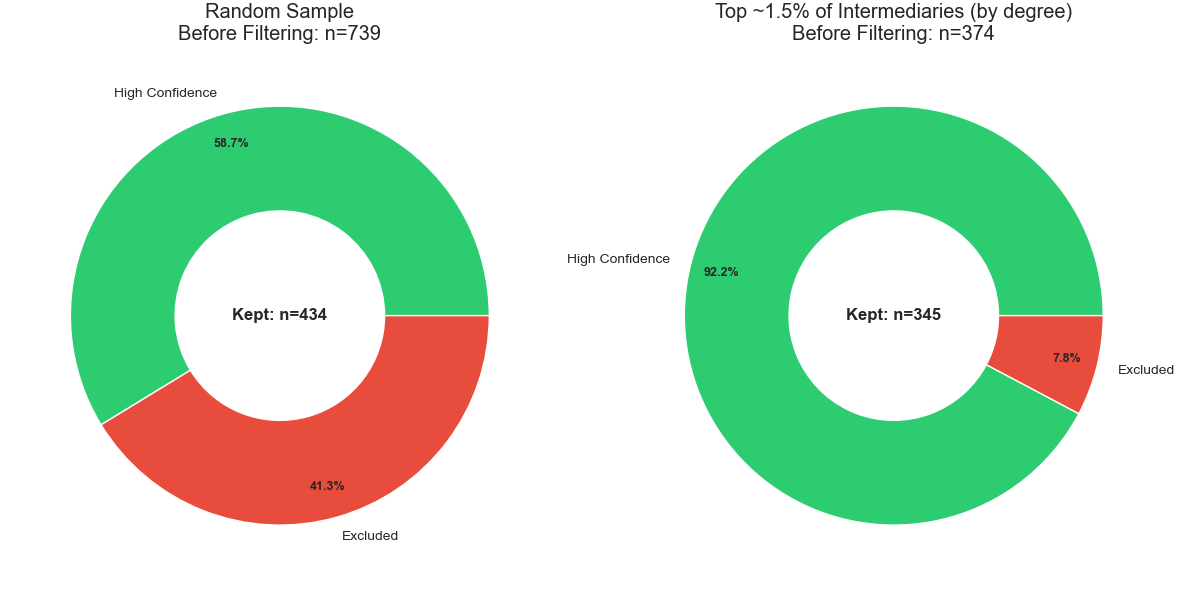
\includegraphics[width=0.8\textwidth]{Appendix_Filtering_of_Enrichment.png}
    \caption{Filtering Process of the Enriched Random Sample for Functional Classification. This flowchart illustrates the steps taken to arrive at the final set of intermediaries with high-confidence functional classifications used in this section's analysis.}
    \label{fig:appendix_filtering_enrichment}
\end{figure}


\section{Replication Code and Classification dataset}

All code to replicate the results as well as all enrichment data classifying the samples of intermediaries can be found here on my GitHub. Link

Note, it can be difficult to navigate the current codebase given the sheer amount of imperative code on there. I've tried keeping it as clean as possible for external eyes as well as documenting continuously, but deadlines caught up with me.






\begin{thebibliography}{99}

\bibitem{Alstadsaeter2019}
Alstads{\ae}ter, A., Johannesen, N., \& Zucman, G. (2019). Tax evasion and inequality. \textit{American Economic Review, 109}(6), 2073–2103. 

\bibitem{Alstadsaeter2022}
Alstadsæter, A., Zucman, G., Planterose, B. \& Økland, A. (2022) Who owns offshore real estate? Evidence from Dubai (EU Tax Observatory working paper 1). https://www.bankofengland.co.uk/-/media/boe/files/events/2022/june/workshop-hf-and-alstadsaeter-paper-2.pdf [Accessed 14th Feburary 2024].

\bibitem{Alstadsaeter2024}
Alstads{\ae}ter, A., Johannesen, N., Le Guern Herry, S., \& Zucman, G. (2024). \textit{Global Tax Evasion Report 2024}. EU Tax Observatory.

\bibitem{Allingham1972}
Allingham, M. G., \& Sandmo, A. (1972). Income tax evasion: A theoretical analysis. \textit{Journal of Public Economics, 1}(3-4), 323–338. 

\bibitem{Angrist2008}
Angrist, J. D., \& Pischke, J.-S. (2008). Mostly harmless econometrics. Princeton University Press.

\bibitem{Blondel2008}
Blondel, V. D., Guillaume, J.-L., Lambiotte, R., \& Lefebvre, E. (2008). Fast unfolding of communities in large networks. \textit{Journal of Statistical Mechanics: Theory and Experiment, 2008}(10), P10008. 

\bibitem{Bourdieu1977}
Bourdieu, P. (1977). \textit{Outline of a theory of practice} (R. Nice, Trans.). Cambridge University Press.

\bibitem{Burke1774}
"Speech of Edmund Burke, Esq. on American taxation, April 19, 1774:." In the digital collection Eighteenth Century Collections Online. https://name.umdl.umich.edu/004902755.0001.000. University of Michigan Library Digital Collections. Accessed May 27, 2025.

\bibitem{Bustos2022}
Bustos, S., Gidi, V., \& Pomeranz, D. (2022). \textit{The race between tax enforcement and tax planning: Evidence from a natural experiment in Chile} (Working Paper).

\bibitem{Carter2017}
Carter, P. (2017). \textit{Why do Development Finance Institutions use offshore financial centres?} Overseas Development Institute.

\bibitem{Chang2023a}
Ho-Chun Herbert Chang, Brooke Harrington, Feng Fu, Daniel N Rockmore, Complex systems of secrecy: the offshore networks of oligarchs, PNAS Nexus, Volume 2, Issue 3, March 2023, pgad051

\bibitem{Chang2023b}
Ho-Chun Herbert Chang, Brooke Harrington, Feng Fu, Daniel N Rockmore (2023). Secrecy Strategies: Global Patterns in Elites' Quest for Confidentiality in Offshore Finance. Presented at The Central Bank of The Bahamas AML/CFT Conference. \url{https://bahamasamlconference.centralbankbahamas.com/documents/2024-03-26-15-06-53-Session-2---Secrecy-Strategies-Global-Patterns-in-Elites-Quest-for-Confidentiality-in-Offshore-Finance.pdf}

\bibitem{Chetty2014}
Chetty, R., Hendren, N., Kline, P., \& Saez, E. (2014). Where is the land of opportunity? The geography of intergenerational mobility in the United States. \textit{The Quarterly Journal of Economics, 129}(4), 1553–1623.

\bibitem{Hearson2020}
Christensen, R.C. \& Hearson, M. (2019) The new politics of global tax governance: taking stock a decade after the financial crisis. Review of International Political Economy, 26(5), 1068–1088. 

\bibitem{Christensen2020}
Christensen, R.C. (2020) Elite professionals in transnational tax governance. Global Networks, 21, 265–293. 

\bibitem{Christensen2024}
Christensen, R. C. (2024). Harnessing network power: Weaponised interdependence in global tax policy. Global Policy.

\bibitem{Christensen2021}
Christensen, R.C., Seabrooke, L. \& Wigan, D. (2021) Professional action in global wealth chains. Regulation \& Governance, 16, 721. 

\bibitem{DeGroen2017}
De Groen, W. P. (2017). Role of advisors and intermediaries in the schemes revealed in the Panama Papers. Directorate-General for Internal Policies. Study for the Pana Committee

\bibitem{Emmenegger2015}
Emmenegger, P. (2015) The long arm of justice: U.S. structural power and international banking. Business \& Politics, 17(3), 473–493. 

\bibitem{Farrell2023}
Farrell, H. \& Newman, A. (2023b) Underground empire: how America weaponized the world economy. London: Allen Lane.

\bibitem{FATF2023}
Financial Action Task Force. (2025). \textit{International standards on combating money laundering and the financing of terrorism \& proliferation: The FATF Recommendations}. FATF. Retrieved from \url{https://www.fatf-gafi.org/en/publications/Fatfrecommendations/Fatf-recommendations.html}

\bibitem{GarciaBernardo2017}
Garcia-Bernardo, J., Fichtner, J., \& Takes, F. W. (2017). Uncovering offshore financial centers: Conduits and sinks in the global corporate ownership network. \textit{Scientific Reports, 7}(1), 6246. 

\bibitem{Granovetter1973}
Granovetter, M. S. (1973). The strength of weak ties. \textit{American Journal of Sociology, 78}(6), 1360–1380. 

\bibitem{Harrington2016}
Harrington, B. (2016). \textit{Capital without borders: Wealth managers and the one percent}. Harvard University Press.

\bibitem{Hastie2009}
Hastie, T., Tibshirani, R., \& Friedman, J. (2009). \textit{The elements of statistical learning: Data mining, inference, and prediction} (2nd ed.). Springer.

\bibitem{Ho2009}
Ho, K. C. (2009). Liquidated. An Ethnography of Wall Street. Duke University Press.

\bibitem{Hoang2022}
Hoang, K. (2022). \textit{Spiderweb Capitalism: How Global Elites Exploit Frontier Markets}. Princeton University Press.

\bibitem{Hoang2020}
Hoang, Kimberly Kay (2020). Engendering Global Capital: How Homoerotic Triangles Facilitate Foreign Investments into Risky Markets. Gender and Society 34 (4):547-572.

\bibitem{ICIJ}
International Consortium of Investigative Journalists. (n.d.). \textit{Offshore Leaks Database}. Retrieved from \url{https://offshoreleaks.icij.org/}

\bibitem{Kejriwal2020}
Kejriwal, S., \& Dang, V. A. (2020). Unveiling the hidden global network of financial secrecy: A panama papers perspective. \textit{EPJ Data Science, 9}(1), 25. 

\bibitem{Kleven2011}
Kleven, H. J., Knudsen, M. B., Kreiner, C. T., Pedersen, S., \& Saez, E. (2011). Unwilling or unable to cheat? Evidence from a tax audit experiment in Denmark. \textit{Econometrica, 79}(3), 651–692. 

\bibitem{Laffitte2024}
Laffitte, S. (2024). \textit{The market for tax havens} [Data set and working paper]. Paris School of Economics.

\bibitem{LondonoVelez2021}
Londo{\~n}o-V{\'e}lez, J., \& {\'A}vila-Mahecha, J. (2021). Enforcing wealth taxes in the developing world: Quasi-experimental evidence from Colombia. \textit{American Economic Review: Insights, 3}(2), 131–148. 

\bibitem{Lowendahl2005}
L{\o}wendahl, B. R. (2005). \textit{Strategic management of professional service firms} (3rd ed.). Copenhagen Business School Press.

\bibitem{Maister1993}
Maister, D. H. (1993). \textit{Managing the professional service firm}. Free Press.

\bibitem{Neely2022}
Neely, M. H. (2022). \textit{Hedged Out: Inequality and Insecurity on Wall Street}. University of California Press.

\bibitem{Newman2010}
Newman, M. E. J. (2010). \textit{Networks: An introduction}. Oxford University Press.

\bibitem{OECD2014}
Organisation for Economic Co-operation and Development. (2014). \textit{Standard for automatic exchange of financial account information in tax matters}. OECD Publishing. 

\bibitem{Palan2002}
Palan, R. (2002). Tax havens and the commercialization of state sovereignty. \textit{International Organization, 56}(1), 151–176. 

\bibitem{Palan2010}
Palan, R., Murphy, R., \& Chavagneux, C. (2010). \textit{Tax havens: How globalization really works}. Cornell University Press.

\bibitem{Piketty2014}
Piketty, T. (2014). \textit{Capital in the twenty-first century} (A. Goldhammer, Trans.). Harvard University Press.

\bibitem{Rixen2010}
Rixen, T. (2010). From double tax avoidance to tax competition: Explaining the institutional trajectory of international tax governance. Review of International Political Economy, 18(2), 197–227. 

\bibitem{Russell1946}
Russell, B. (1946). \textit{History of Western philosophy}. George Allen \& Unwin.

\bibitem{Saez2019}
Saez, E., \& Zucman, G. (2019). \textit{The triumph of injustice: How the rich dodge taxes and how to make them pay}. W. W. Norton \& Company.

\bibitem{Seabrooke2017}
Seabrooke, L., \& Wigan, D. (2017). The governance of global wealth chains. \textit{Review of International Political Economy, 24}(1), 1-29. 

\bibitem{Shiller2012}
Shiller, R. J. (2012). \textit{Finance and the good society}. Princeton University Press.

\bibitem{Slemrod2019}
Slemrod, J. (2019). Tax Compliance and Enforcement: New Developments. \textit{Journal of Economic Literature, 57}, 907-954. 

\bibitem{Stausholm2024}
Stausholm, S. \& Garcia-Bernardo, J. (2024) Unfollow the money: mapping the micro agents of international tax. Review of International Political Economy, 31(4), 1197–1219. 

\bibitem{Stiglitz2025}
Stiglitz, J. E. (2025, April). America Is becoming the World's Largest Tax Haven \textit{Project Syndicate}. Retrieved from \url{https://www.project-syndicate.org/commentary/america-becoming-largest-tax-haven-under-trump-by-joseph-e-stiglitz-2025-04}

\bibitem{TJN2022}
Tax Justice Network. (2022). Financial Secrecy Index 2022. Tax Justice Network. https://fsi.taxjustice.net/

\bibitem{Tilly1990}
Tilly, C. (1990). \textit{Coercion, capital, and European states, AD 990-1990}. Basil Blackwell.

\bibitem{Torslov2018}
T{\o}rsl{\o}v, T. R., Wier, L. S., \& Zucman, G. (2018). \textit{The missing profits of nations} (NBER Working Paper No. 24701). National Bureau of Economic Research. 

\bibitem{Vdem2023}
Varieties of Democracy (V-Dem) Institute. (2023). \textit{V-Dem Dataset v13}. Retrieved from \url{https://www.v-dem.net/data/the-v-dem-dataset/}

\bibitem{vonNordenflycht2010}
von Nordenflycht, A. (2010). What is a professional service firm? Toward a theory and taxonomy of knowledge-intensive firms. \textit{Academy of Management Review, 35}(1), 155–174. \url{https://doi.org/10.5465/amr.35.1.zok155}

\bibitem{Wei2024}
Wei, X. (2024). \textit{The development of Hong Kong as an intermediate financial centre after 1978, by studying Chinese state-owned banks in Hong Kong} (Unpublished doctoral thesis). City, University of London.

\bibitem{Weinberg2023}
ICIJ. \textit{Cyprus confidential}. International Consortium of Investigative Journalists. Retrieved from \url{https://www.icij.org/investigations/cyprus-confidential/}

\bibitem{Zar2010}
Zar, J.H. (2010) Biostatistical Analysis. 5th Edition, Prentice-Hall/Pearson

\bibitem{Zucman2015}
Zucman, G. (2015) The hidden wealth of nations: the scourge of tax havens. Chicago: University of Chicago Press.

\end{thebibliography}



% Word count: texcount -inc main.tex -sum -char
%TC:endignore

\end{document}
% --- Document End ---
